% !TEX root=../../mt-motion-analysis.tex
% \newpage
\appendix
% \newpage
% \etocdepthtag.toc{mtappendix}
% \etocsettagdepth{mtchapter}{none}
% \etocsettagdepth{mtappendix}{subsection}
% \etoctocstyle{1}{Appendix - Contents}
% \tableofcontents
% \newpage


\chapter[POE-task combinations]{POE-task combinations \cite{Nae2020b}} \label{app:poe-task}
% {\floatsep=0
% lol
% \begin{figure}
  \begin{center}
    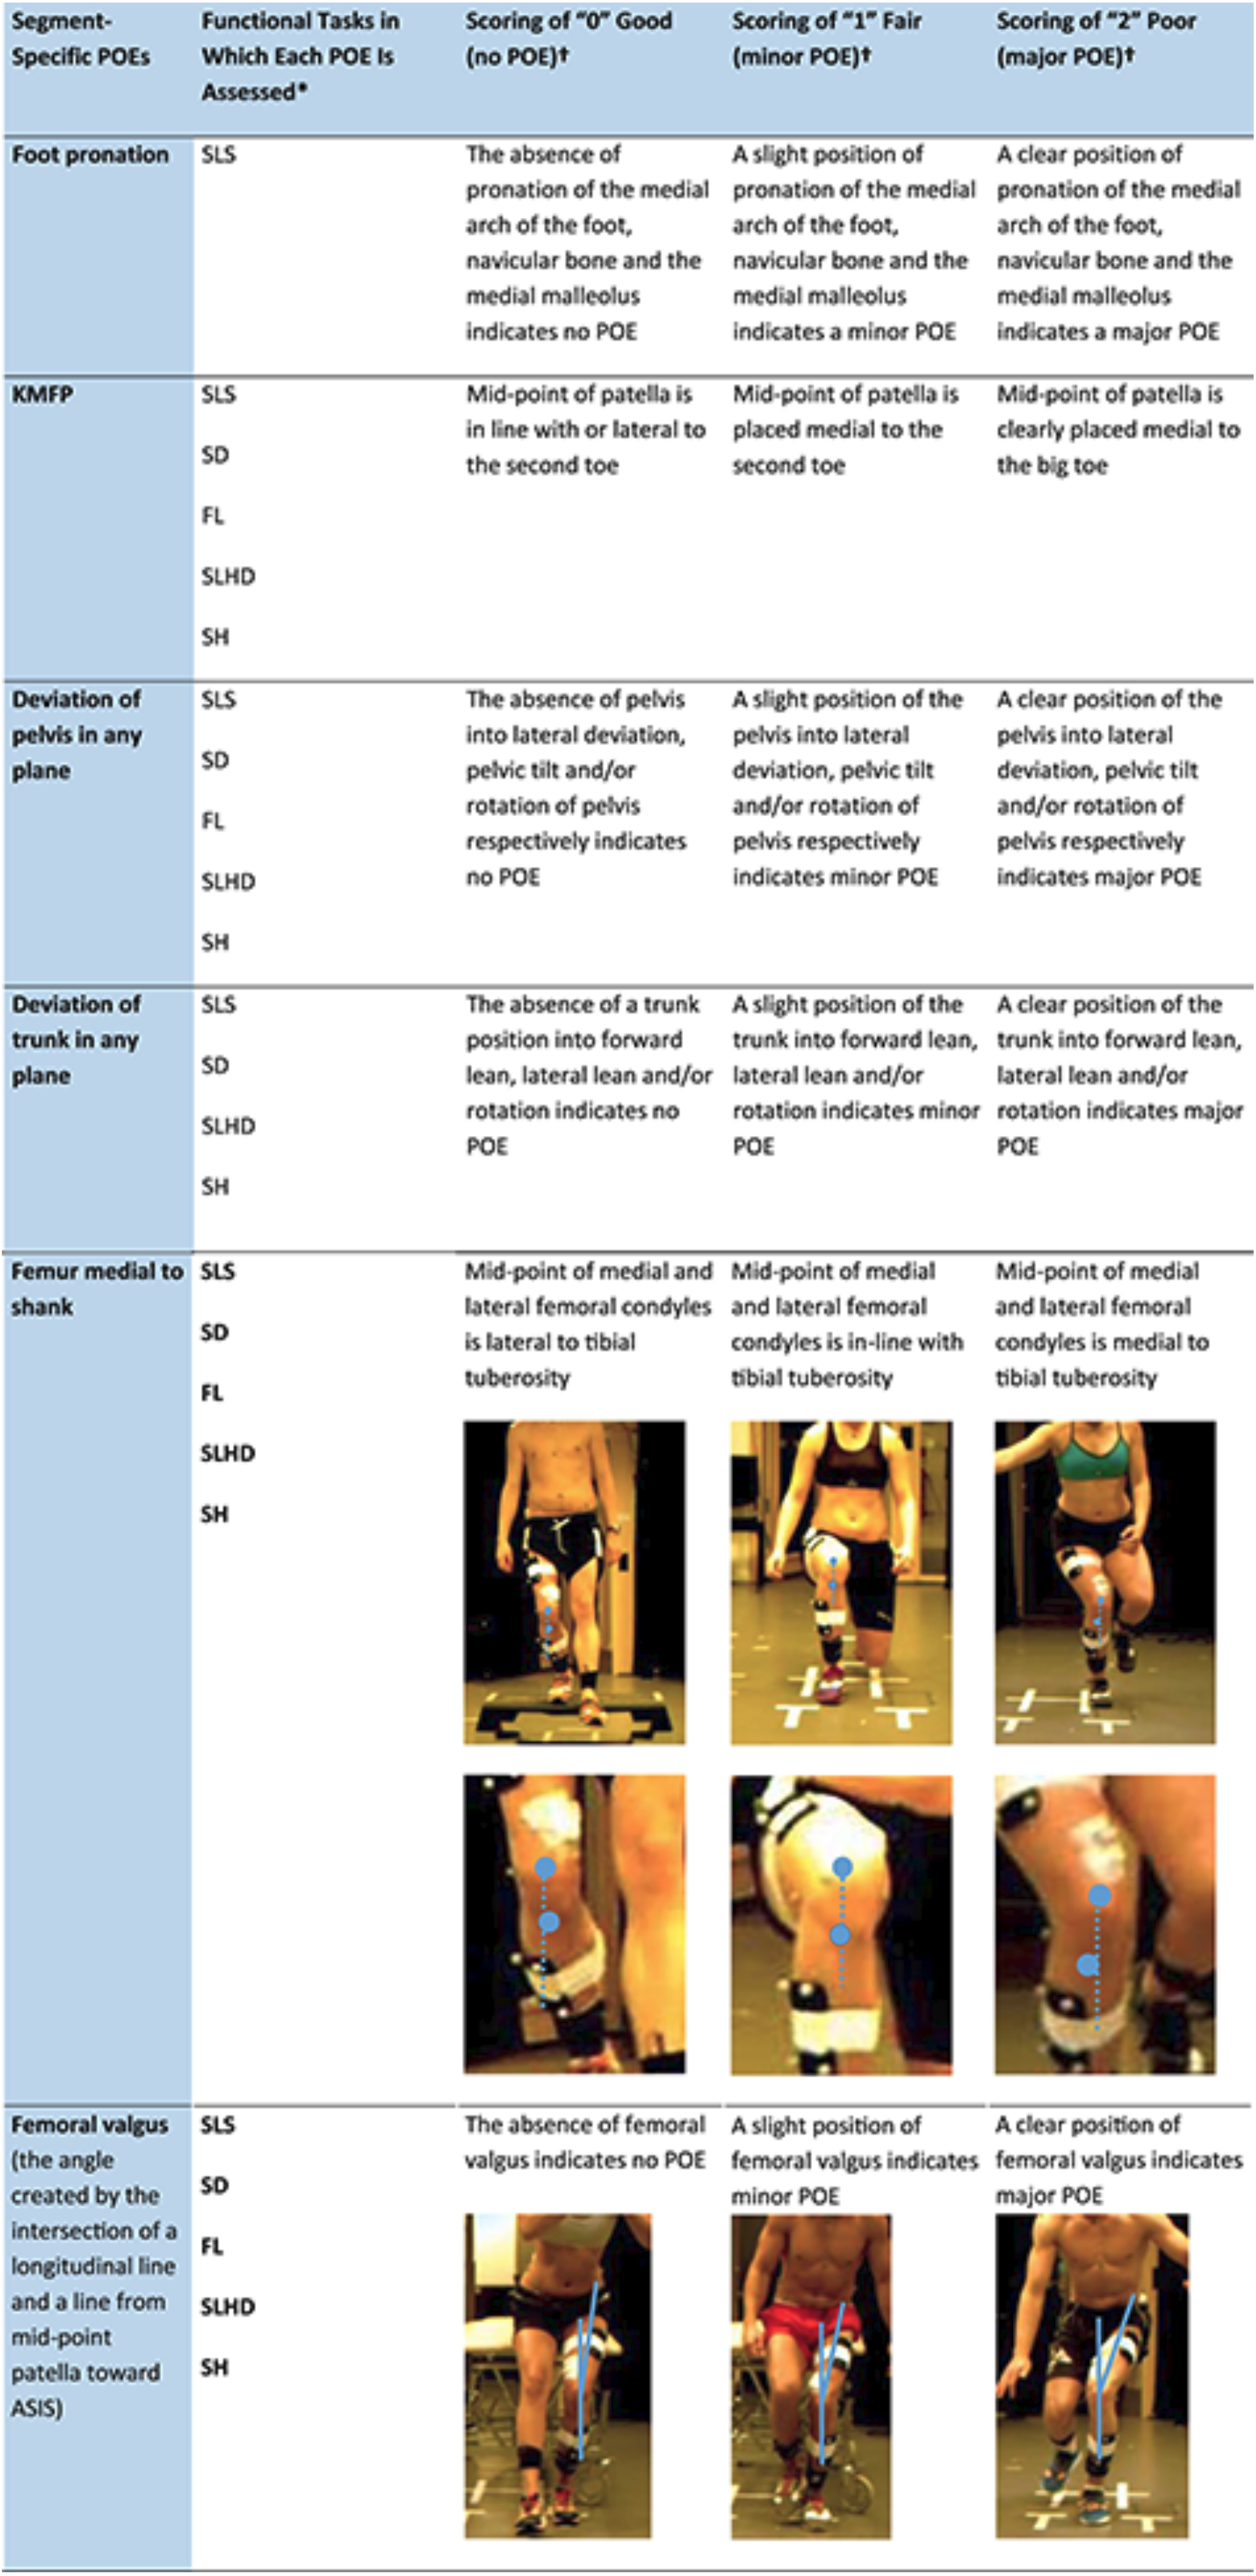
\includegraphics[trim=0 60 0 0, clip, height=0.9\textheight]{files/figs/app/poes-detailed-rot.png}
  \end{center}
  % \caption{}
  % \label{}
% \end{figure}
% }
 % over probabilities on validation sets
 \chapter{Models} \label{app:models}
 \section{Trunk}
 \begin{center}
   \footnotesize
   \setlength\arraycolsep{2pt}
   \begin{tabu}[c]{|c|c|c|c|c|c|}
     \hline
     & \textbf{T1} & \textbf{T2} & \textbf{T3} & \textbf{T4} & \textbf{T5} \\\hline
     \multicolumn{1}{|c|}{\begin{tabular}[c]{@{}c@{}}\textbf{Training}\\\textbf{weights}\end{tabular}} &
     $\begin{bmatrix}1 & 5 \end{bmatrix}$ & $\begin{bmatrix}1 & 5 \end{bmatrix}$ &
     $\begin{bmatrix}0.6 & 0.04 & 0.04 \\ 0 & 1 & 1 \\ 0 & 1 & 1 \end{bmatrix}$ &
     $\begin{bmatrix}1 & 0 & 0 \\ 0.3 & 0.45 & 0.3 \\ 0 & 0 & 1 \end{bmatrix}$ &
     $\begin{bmatrix}1 & 10 \end{bmatrix}$ \\ \hline
     \multicolumn{1}{|c|}{\begin{tabular}[c]{@{}c@{}}\textbf{Ensemble}\\\textbf{weights}\end{tabular}}&
     $\begin{bmatrix}1/3 & 1.15/3 & 1/3 \end{bmatrix}$ & $\begin{bmatrix}1/3 & 1.15/3 & 1/3 \end{bmatrix}$ &
     $\begin{bmatrix}1/3 & 0 & 0 \end{bmatrix}$ & $\begin{bmatrix}0 & 1.15/3 & 0 \end{bmatrix}$ &
     $\begin{bmatrix}0 & 0 & 1/3 \end{bmatrix}$ \\ \hline
     \multicolumn{1}{|c|}{\begin{tabular}[c]{@{}c@{}}\textbf{Trainable}\\\textbf{parameters}\end{tabular}}& 197890 & 197890 & 47747 & 119879 & 47651 \\ \hline
   \end{tabu}
\end{center}

\section{Pelvis}
\begin{center}
  \footnotesize
  \setlength\arraycolsep{2pt}
  \begin{tabu}[c]{|c|c|c|c|c|c|}
    \hline
    & \textbf{P1} & \textbf{P2} & \textbf{P3} & \textbf{P4} & \textbf{P5} \\\hline
    \multicolumn{1}{|c|}{\begin{tabular}[c]{@{}c@{}}\textbf{Training}\\\textbf{weights}\end{tabular}} &
    $\begin{bmatrix}2 & 1 \end{bmatrix}$ & $\begin{bmatrix}2 & 1 \end{bmatrix}$ &
    $\begin{bmatrix}0.6 & 0.04 & 0.04 \\ 0 & 1 & 1 \\ 0 & 1 & 1 \end{bmatrix}$ &
    $\begin{bmatrix}1 & 0 & 0 \\ 0.3 & 0.45 & 0.3 \\ 0 & 0 & 1 \end{bmatrix}$ &
    $\begin{bmatrix}1 & 5 \end{bmatrix}$ \\ \hline
    \multicolumn{1}{|c|}{\begin{tabular}[c]{@{}c@{}}\textbf{Ensemble}\\\textbf{weights}\end{tabular}}&
    $\begin{bmatrix}1/3 & 1.05/3 & 1/3 \end{bmatrix}$ & $\begin{bmatrix}1/3 & 1.05/3 & 1/3 \end{bmatrix}$ &
    $\begin{bmatrix}1/3 & 0 & 0 \end{bmatrix}$ & $\begin{bmatrix}0 & 1.05/3 & 0 \end{bmatrix}$ &
    $\begin{bmatrix}0 & 0 & 1/3 \end{bmatrix}$ \\ \hline
    \multicolumn{1}{|c|}{\begin{tabular}[c]{@{}c@{}}\textbf{Trainable}\\\textbf{parameters}\end{tabular}}& 183044 & 183044 & 112577 & 112577 & 41543 \\ \hline
  \end{tabu}
\end{center}

\section{Femoral Valgus}
\begin{center}
  \footnotesize
  \setlength\arraycolsep{2pt}
  \begin{tabu}[c]{|c|c|c|c|c|c|}
    \hline
    & \textbf{F1} & \textbf{F2} & \textbf{F3} & \textbf{F4} & \textbf{F5} \\\hline
    \multicolumn{1}{|c|}{\begin{tabular}[c]{@{}c@{}}\textbf{Training}\\\textbf{weights}\end{tabular}} &
    $\begin{bmatrix}1 & 1 \end{bmatrix}$ & $\begin{bmatrix}1 & 1 \end{bmatrix}$ &
    $\begin{bmatrix}0.6 & 0.04 & 0.04 \\ 0 & 1 & 1 \\ 0 & 1 & 1 \end{bmatrix}$ &
    $\begin{bmatrix}1 & 0 & 0 \\ 0.3 & 0.45 & 0.3 \\ 0 & 0 & 1 \end{bmatrix}$ &
    $\begin{bmatrix}1 & 1 & 0 \\ 1 & 1 & 0 \\ 0.1 & 0.1 & 0.6 \end{bmatrix}$ \\ \hline
    \multicolumn{1}{|c|}{\begin{tabular}[c]{@{}c@{}}\textbf{Ensemble}\\\textbf{weights}\end{tabular}}&
    $\begin{bmatrix}1/3 & 1.25/3 & 1/3 \end{bmatrix}$ & $\begin{bmatrix}1/3 & 1.25/3 & 1/3 \end{bmatrix}$ &
    $\begin{bmatrix}1/3 & 0 & 0 \end{bmatrix}$ & $\begin{bmatrix}0 & 1.25/3 & 0 \end{bmatrix}$ &
    $\begin{bmatrix}0 & 0 & 1/3 \end{bmatrix}$ \\ \hline
    \multicolumn{1}{|c|}{\begin{tabular}[c]{@{}c@{}}\textbf{Trainable}\\\textbf{parameters}\end{tabular}}& 90648 & 23720 & 23727 & 23727 & 23727 \\ \hline
  \end{tabu}
\end{center}

\section{Knee Medial-to-Foot-Position} \label{app:models-kmfp}
\begin{center}
  \footnotesize
  \setlength\arraycolsep{2pt}
  \begin{tabu}[c]{|c|c|c|c|c|c|}
    \hline
    & \textbf{K1} & \textbf{K2} & \textbf{K3} & \textbf{K4} & \textbf{K5} \\\hline
    \multicolumn{1}{|c|}{\begin{tabular}[c]{@{}c@{}}\textbf{Training}\\\textbf{weights}\end{tabular}} &
    $\begin{bmatrix}1 & 1 & 1 \end{bmatrix}$ & $\begin{bmatrix}1 & 1 & 1 \end{bmatrix}$ &
    $\begin{bmatrix}0.6 & 0.04 & 0.04 \\ 0 & 1 & 1 \\ 0 & 1 & 1 \end{bmatrix}$ &
    $\begin{bmatrix}1 & 0 & 0 \\ 0.3 & 0.45 & 0.3 \\ 0 & 0 & 1 \end{bmatrix}$ &
    $\begin{bmatrix}1 & 1 & 0 \\ 1 & 1 & 0 \\ 0.05 & 0.05 & 0.7 \end{bmatrix}$ \\ \hline
    \multicolumn{1}{|c|}{\begin{tabular}[c]{@{}c@{}}\textbf{Ensemble}\\\textbf{weights}\end{tabular}}&
    $\begin{bmatrix}1/3 & 1.25/3 & 1/3 \end{bmatrix}$ & $\begin{bmatrix}1/3 & 1.25/3 & 1/3 \end{bmatrix}$ &
    $\begin{bmatrix}1/3 & 0 & 0 \end{bmatrix}$ & $\begin{bmatrix}0 & 1.25/3 & 0 \end{bmatrix}$ &
    $\begin{bmatrix}0 & 0 & 1/3 \end{bmatrix}$ \\ \hline
    \multicolumn{1}{|c|}{\begin{tabular}[c]{@{}c@{}}\textbf{Trainable}\\\textbf{parameters}\end{tabular}}& 168195 & 35843 & 35843 & 105265 & 35843 \\ \hline
  \end{tabu}
\end{center}

\chapter{Histograms over probabilities on validation sets} \label{app:val-hists}
\section{Trunk}
The first row shows all the predicted probabilities for the different classes. The second row shows the probabilities for the predicted class for all repetitions, i.e. the histograms of the highest probabilities for the different classes for all repetitions. The third and fourth rows show the corresponding histograms for the combined scores.

\begin{center}
\begin{minipage}{0.33\textwidth}
  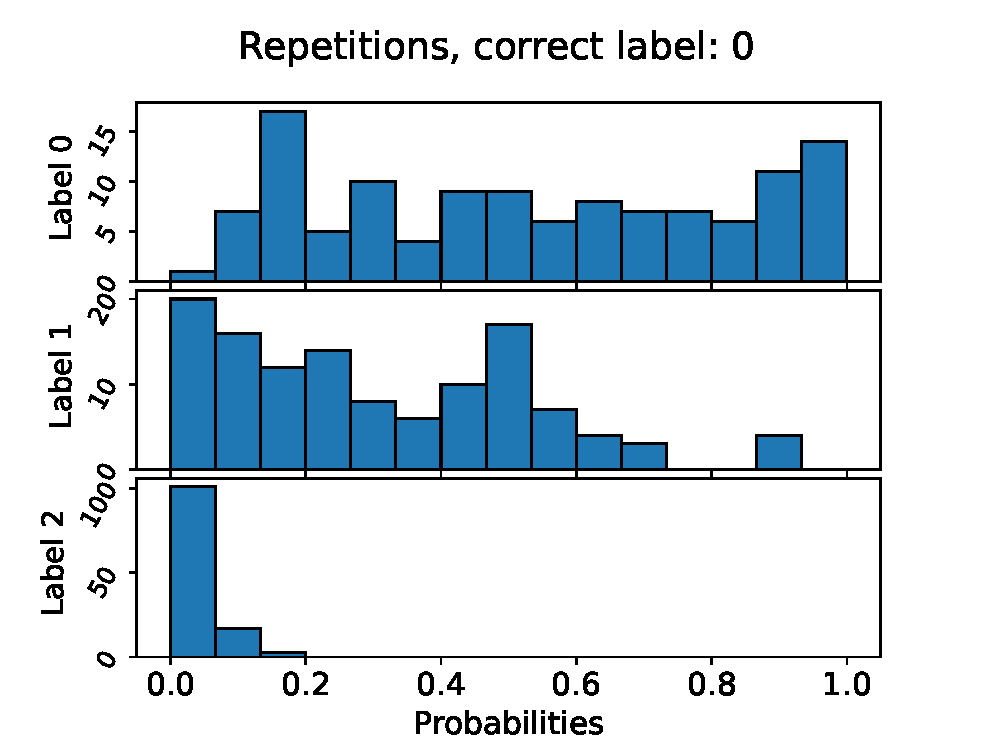
\includegraphics[width=\textwidth]{files/figs/app/hists/trunk/r0.eps}
\end{minipage}%
\begin{minipage}{0.33\textwidth}
  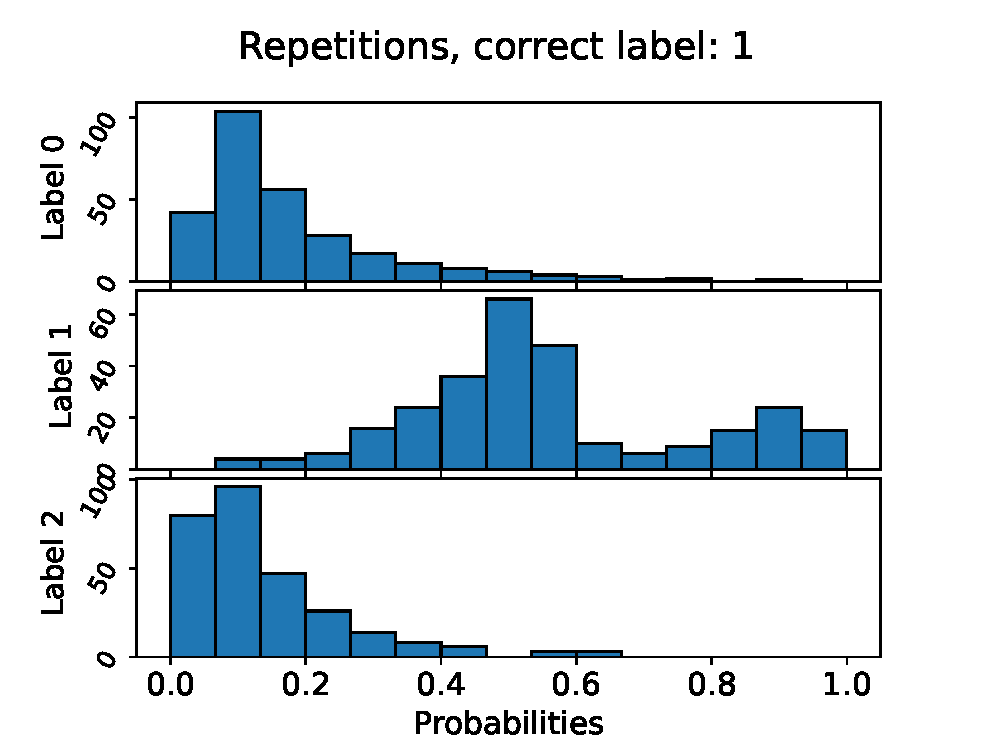
\includegraphics[width=\textwidth]{files/figs/app/hists/trunk/r1.eps}
\end{minipage}%
\begin{minipage}{0.33\textwidth}
  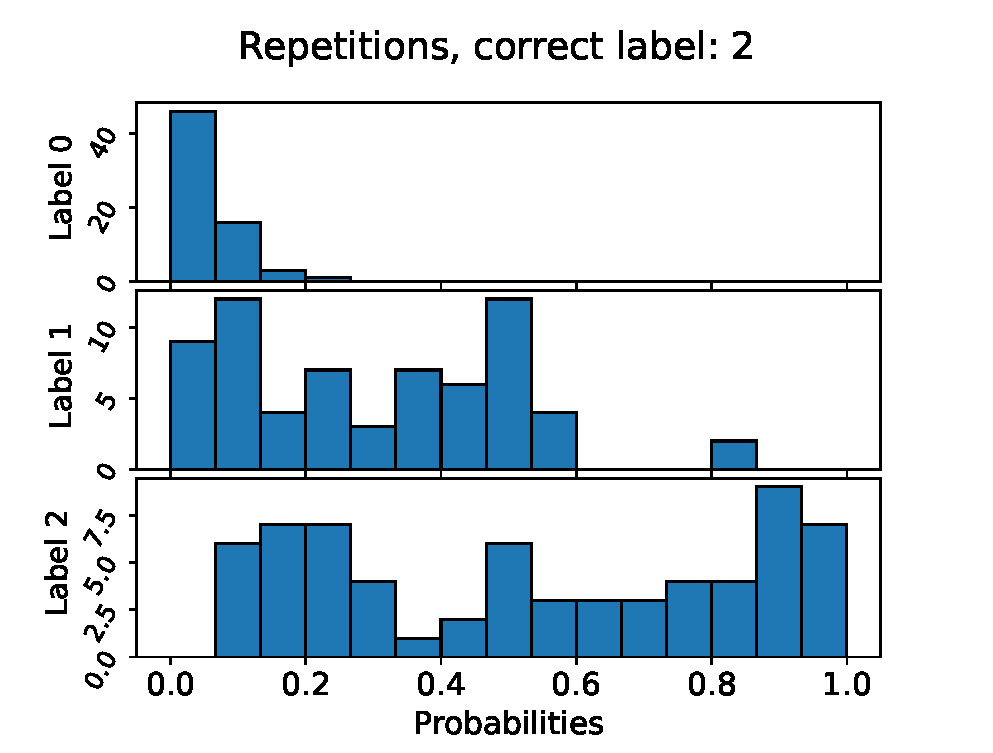
\includegraphics[width=\textwidth]{files/figs/app/hists/trunk/r2.eps}
\end{minipage}

\begin{minipage}{0.33\textwidth}
  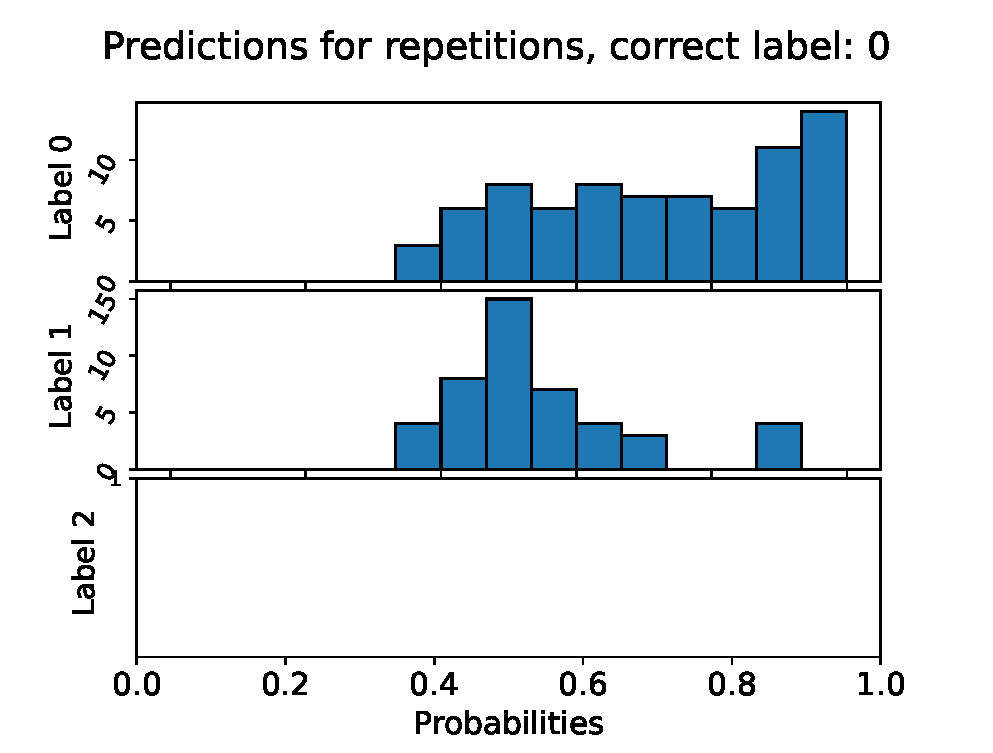
\includegraphics[width=\textwidth]{files/figs/app/hists/trunk/pr0.eps}
\end{minipage}%
\begin{minipage}{0.33\textwidth}
  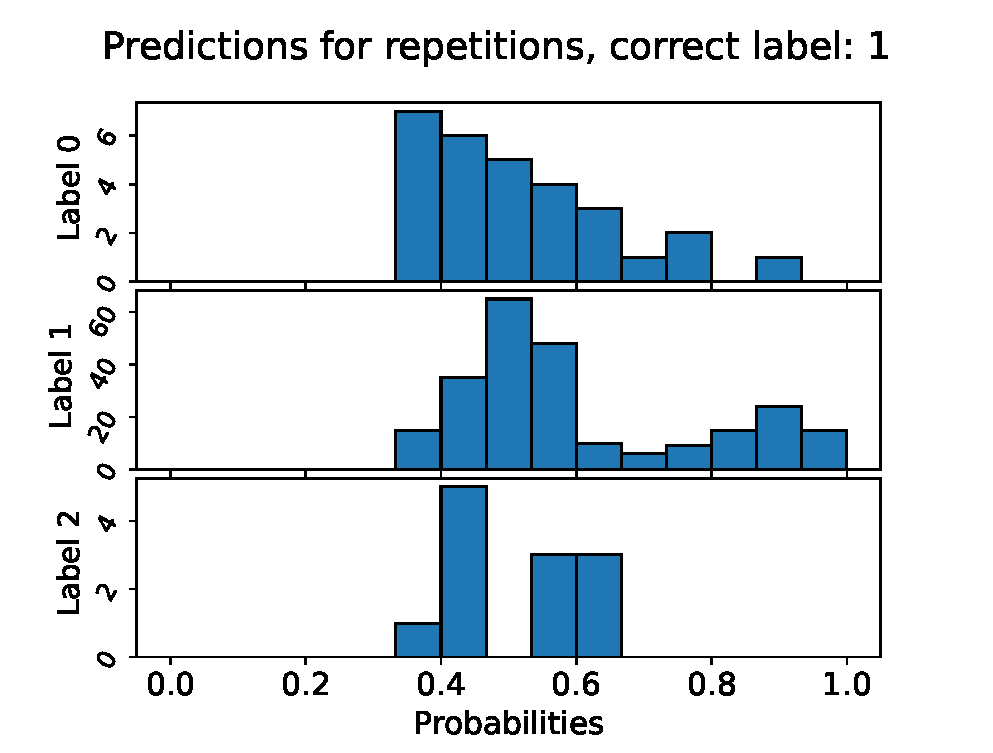
\includegraphics[width=\textwidth]{files/figs/app/hists/trunk/pr1.eps}
\end{minipage}%
\begin{minipage}{0.33\textwidth}
  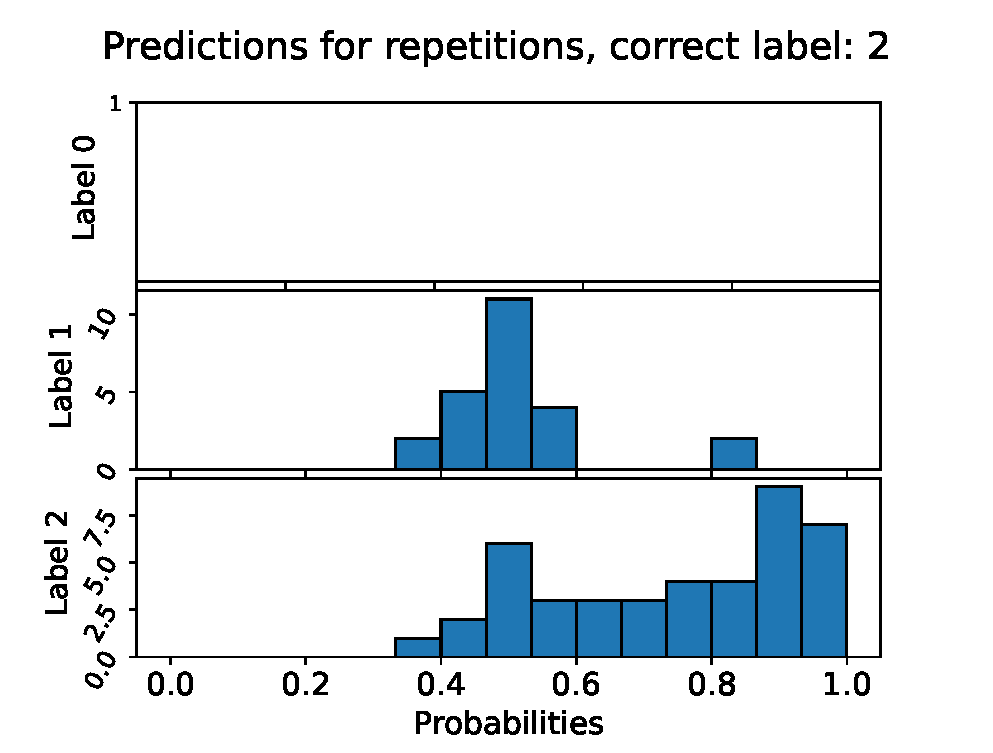
\includegraphics[width=\textwidth]{files/figs/app/hists/trunk/pr2.eps}
\end{minipage}

\begin{minipage}{0.33\textwidth}
  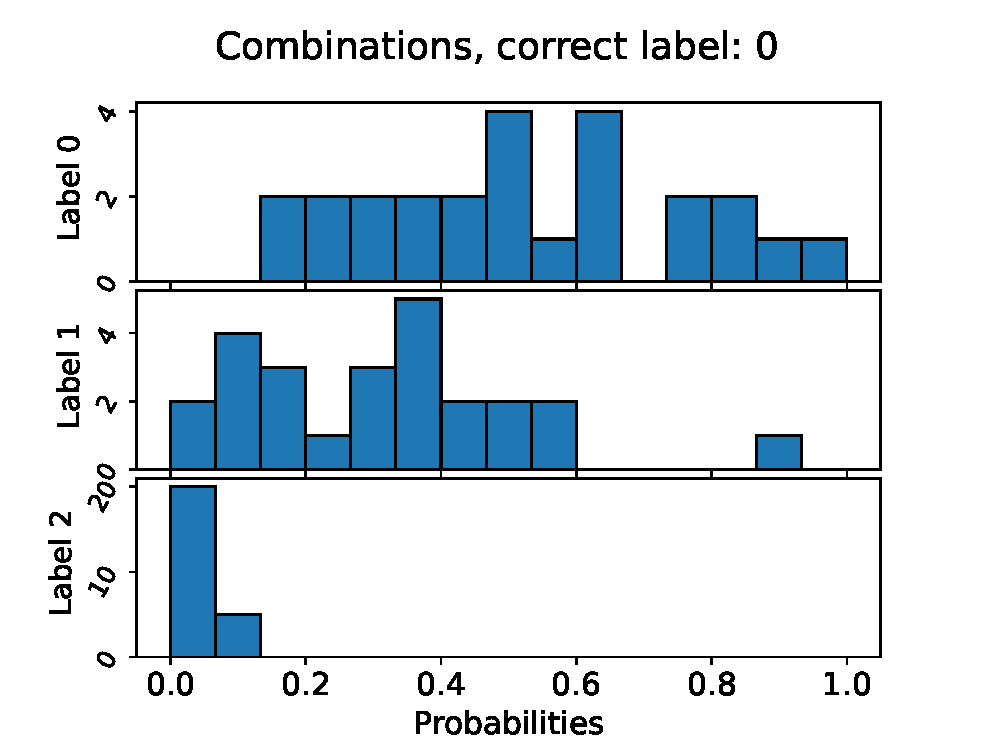
\includegraphics[width=\textwidth]{files/figs/app/hists/trunk/c0.eps}
\end{minipage}%
\begin{minipage}{0.33\textwidth}
  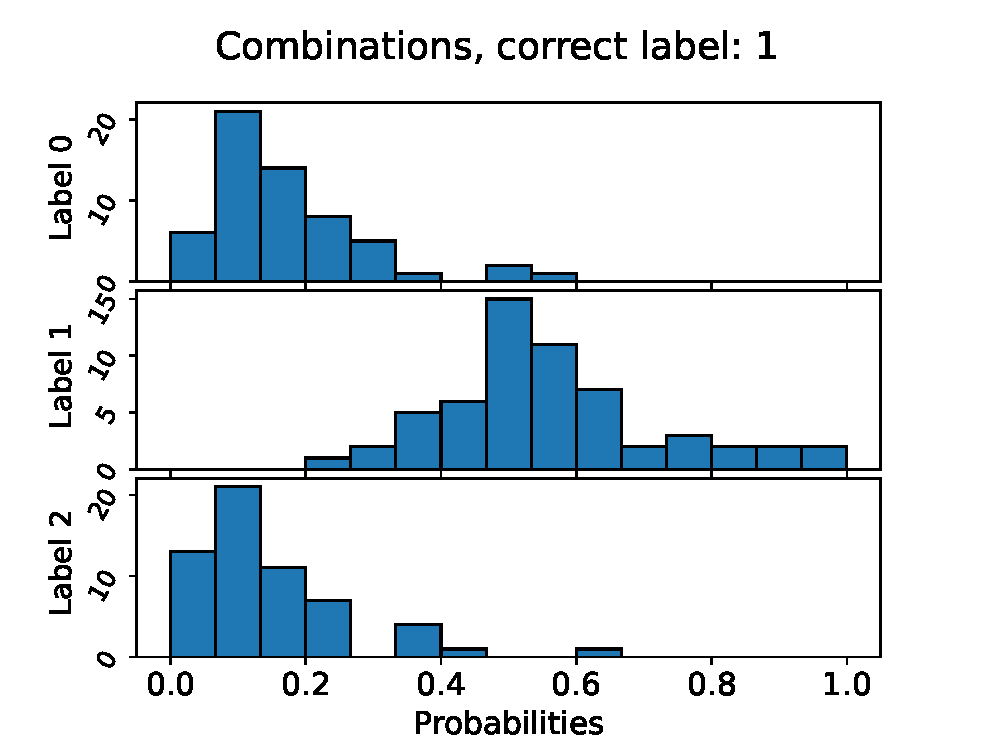
\includegraphics[width=\textwidth]{files/figs/app/hists/trunk/c1.eps}
\end{minipage}%
\begin{minipage}{0.33\textwidth}
  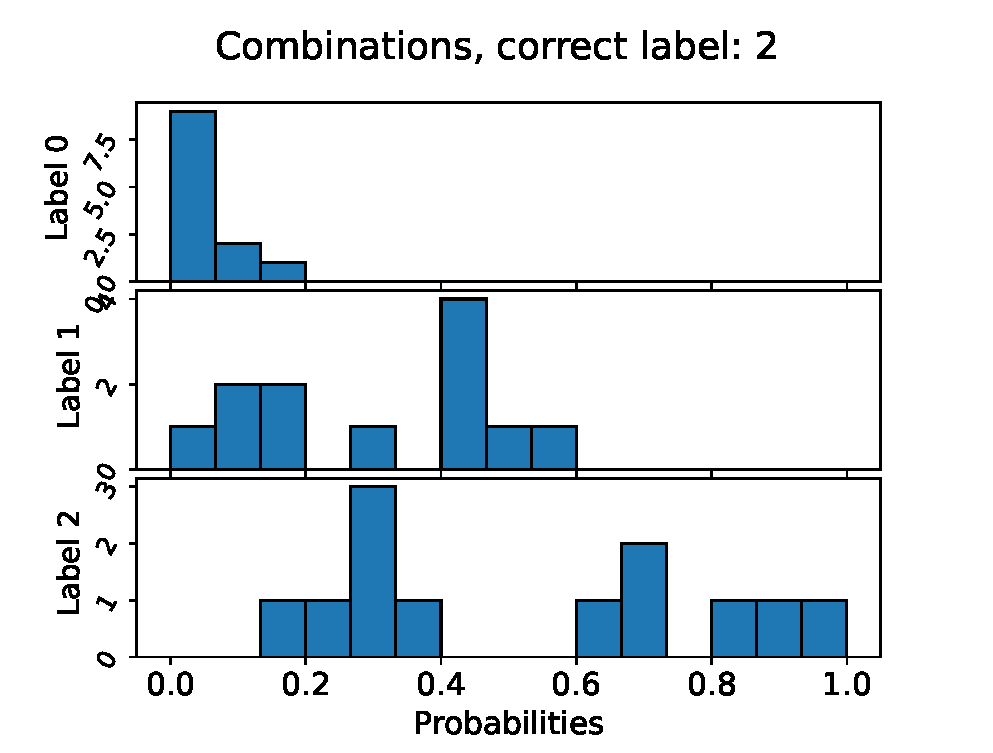
\includegraphics[width=\textwidth]{files/figs/app/hists/trunk/c2.eps}
\end{minipage}

\begin{minipage}{0.33\textwidth}
  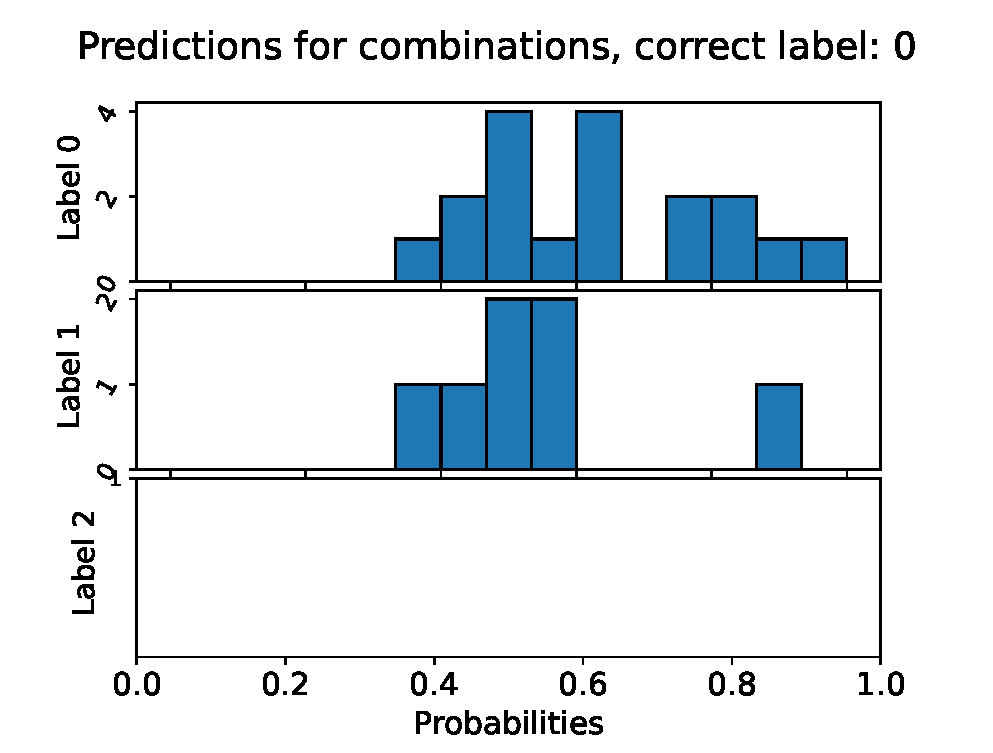
\includegraphics[width=\textwidth]{files/figs/app/hists/trunk/pc0.eps}
\end{minipage}%
\begin{minipage}{0.33\textwidth}
  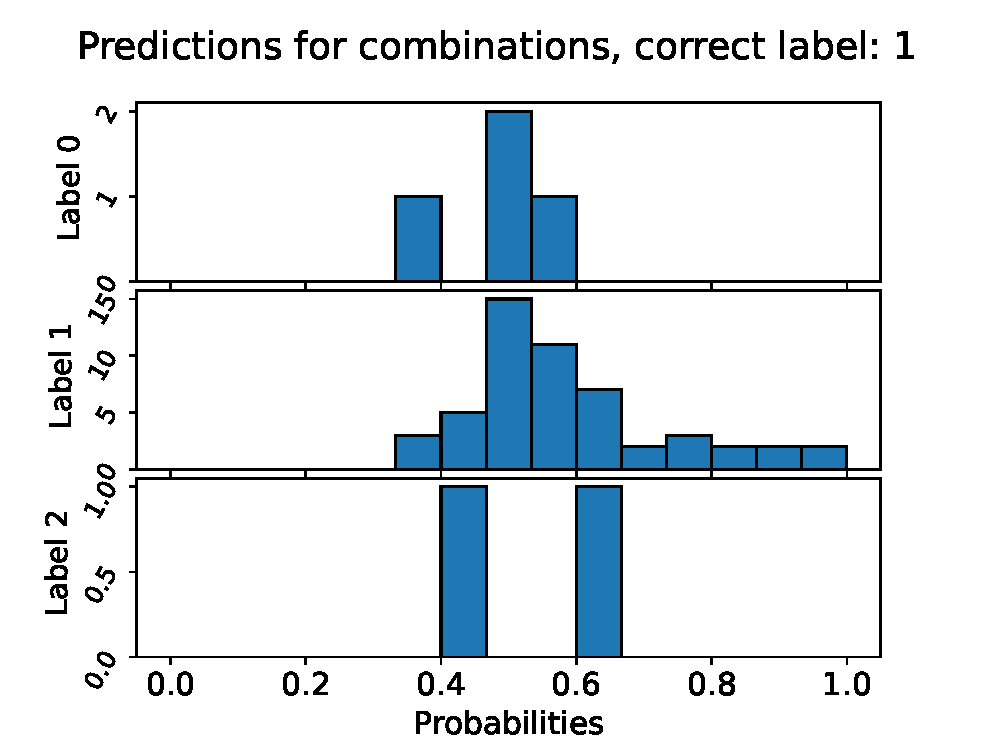
\includegraphics[width=\textwidth]{files/figs/app/hists/trunk/pc1.eps}
\end{minipage}%
\begin{minipage}{0.33\textwidth}
  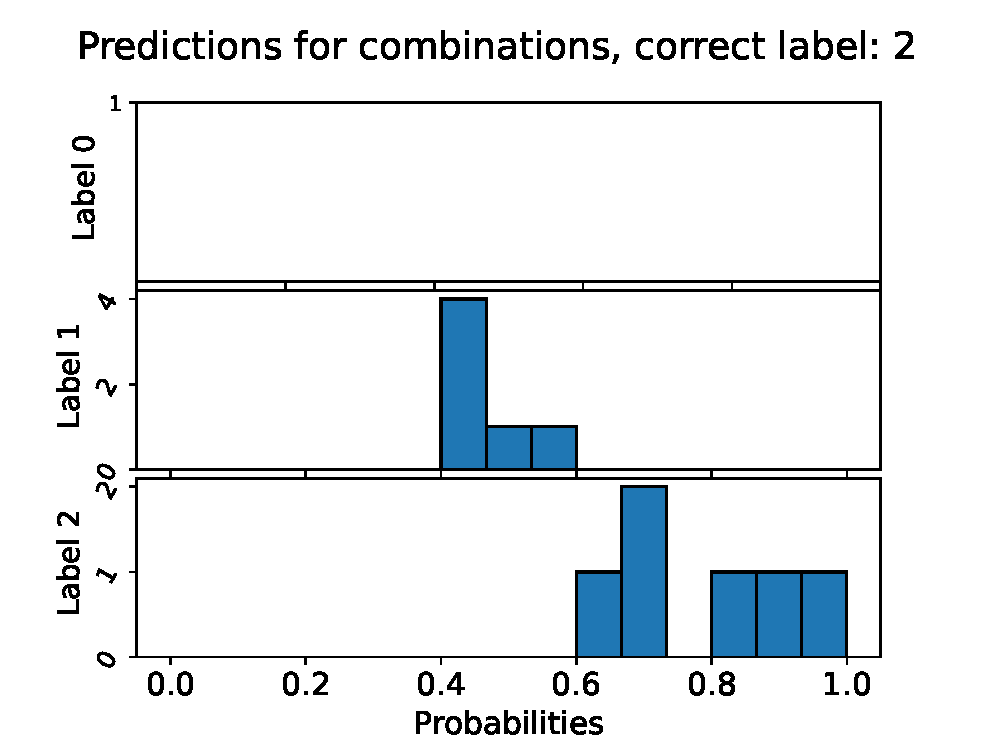
\includegraphics[width=\textwidth]{files/figs/app/hists/trunk/pc2.eps}
\end{minipage}
\end{center}

\newpage
\section{Pelvis}
The first row shows all the predicted probabilities for the different classes. The second row shows the probabilities for the predicted class for all repetitions, i.e. the histograms of the highest probabilities for the different classes for all repetitions. The third and fourth rows show the corresponding histograms for the combined scores.

\begin{center}
\begin{minipage}{0.33\textwidth}
  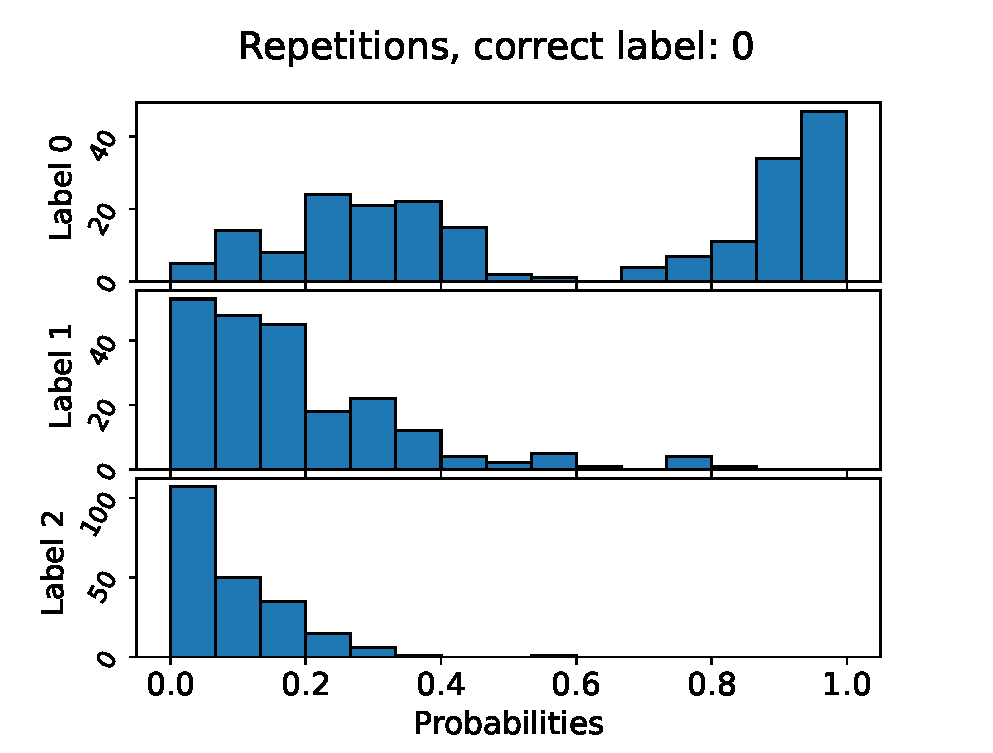
\includegraphics[width=\textwidth]{files/figs/app/hists/pelvis/r0.eps}
\end{minipage}%
\begin{minipage}{0.33\textwidth}
  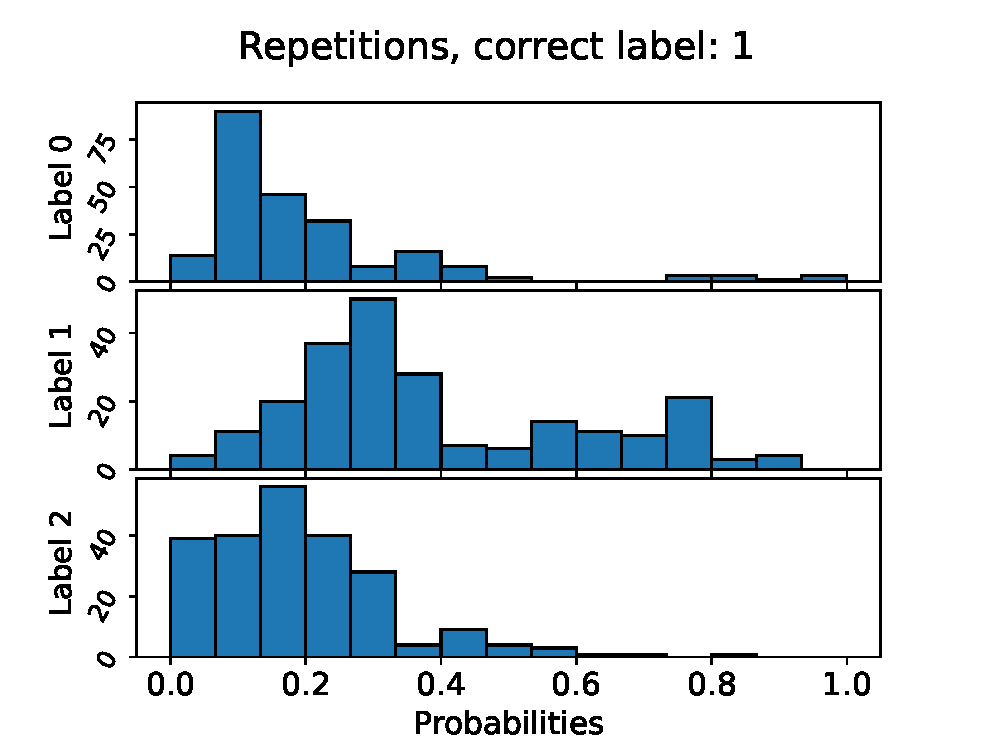
\includegraphics[width=\textwidth]{files/figs/app/hists/pelvis/r1.eps}
\end{minipage}%
\begin{minipage}{0.33\textwidth}
  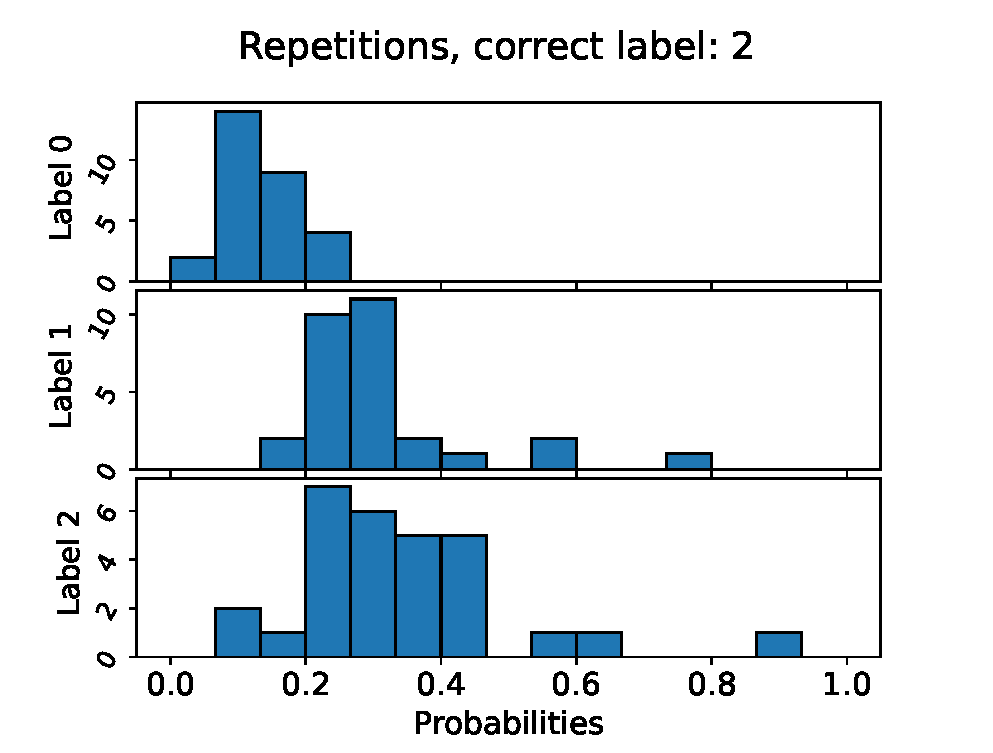
\includegraphics[width=\textwidth]{files/figs/app/hists/pelvis/r2.eps}
\end{minipage}

\begin{minipage}{0.33\textwidth}
  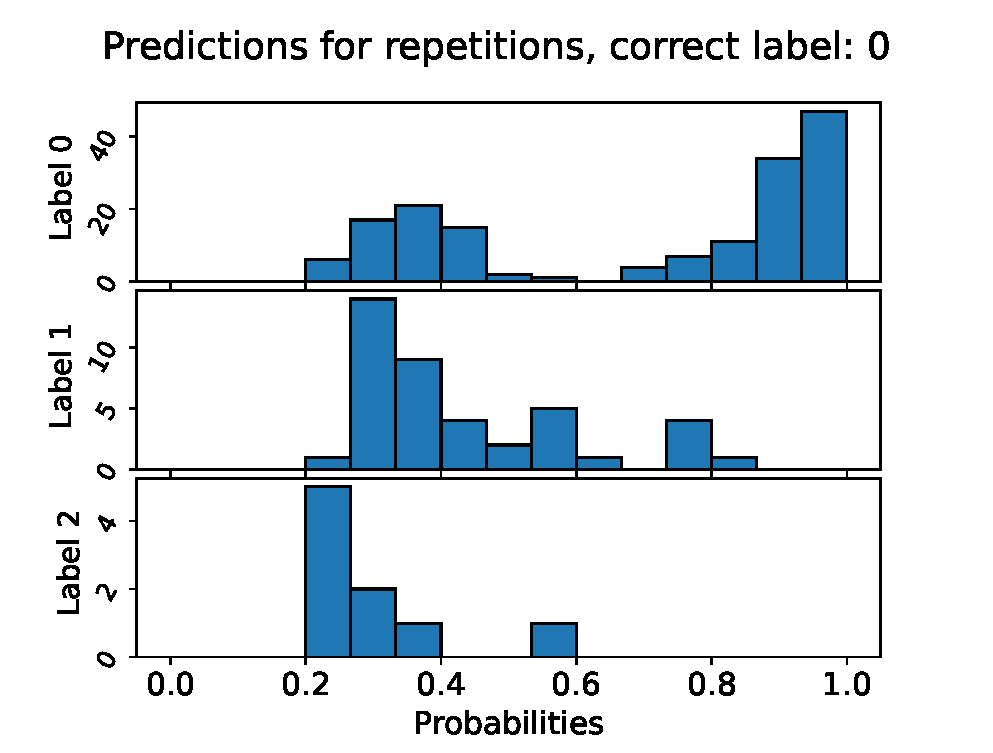
\includegraphics[width=\textwidth]{files/figs/app/hists/pelvis/pr0.eps}
\end{minipage}%
\begin{minipage}{0.33\textwidth}
  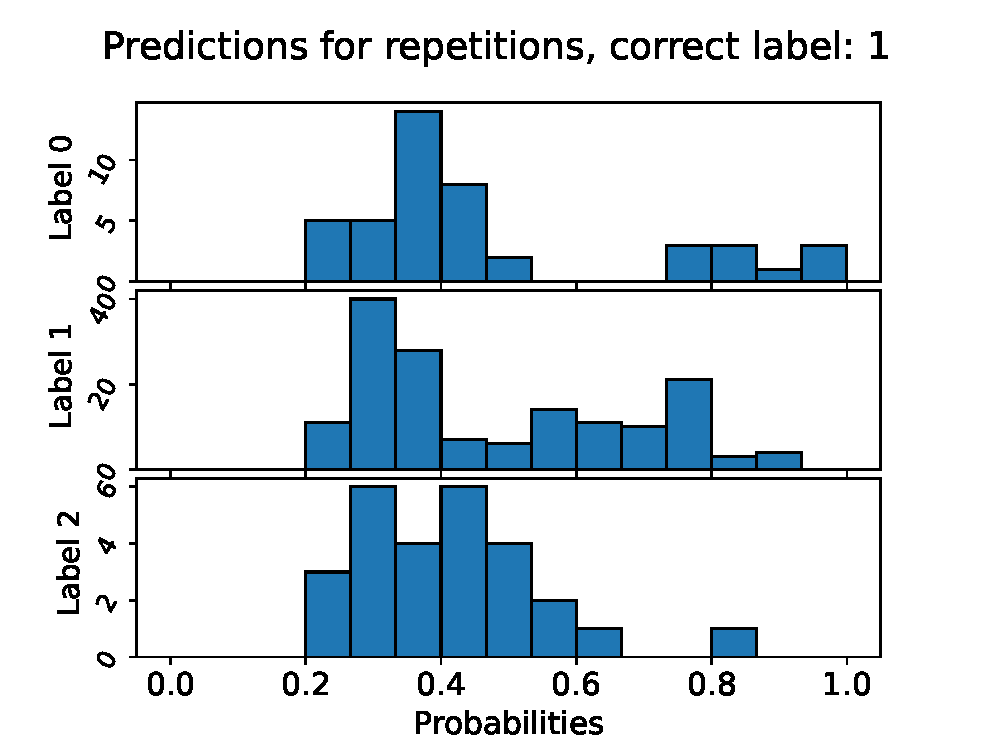
\includegraphics[width=\textwidth]{files/figs/app/hists/pelvis/pr1.eps}
\end{minipage}%
\begin{minipage}{0.33\textwidth}
  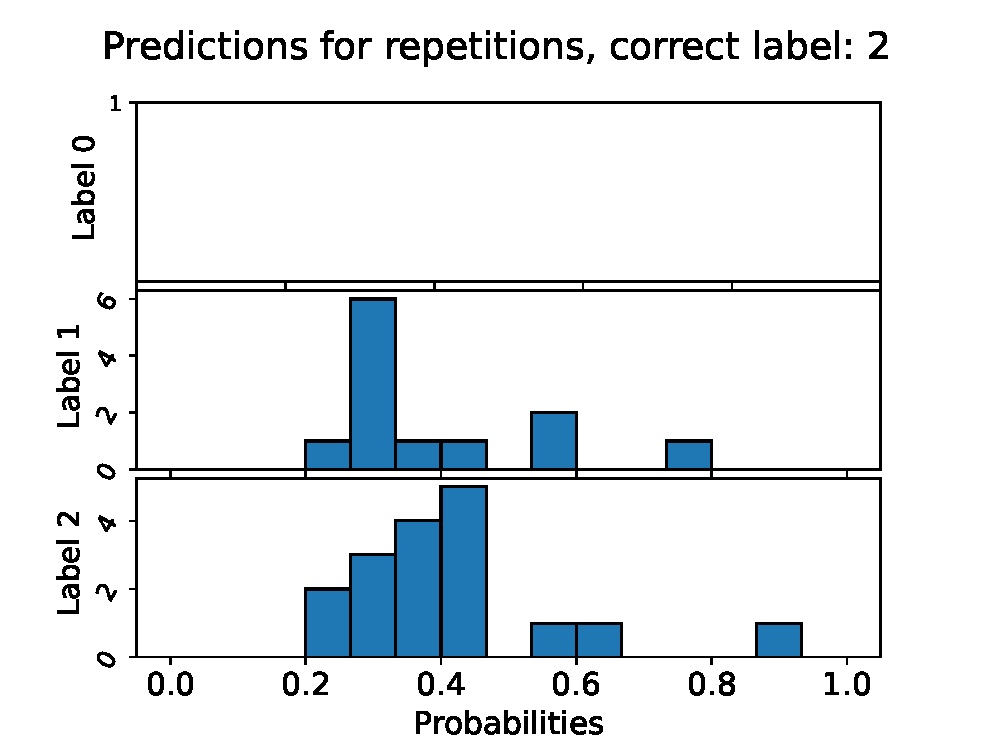
\includegraphics[width=\textwidth]{files/figs/app/hists/pelvis/pr2.eps}
\end{minipage}

\begin{minipage}{0.33\textwidth}
  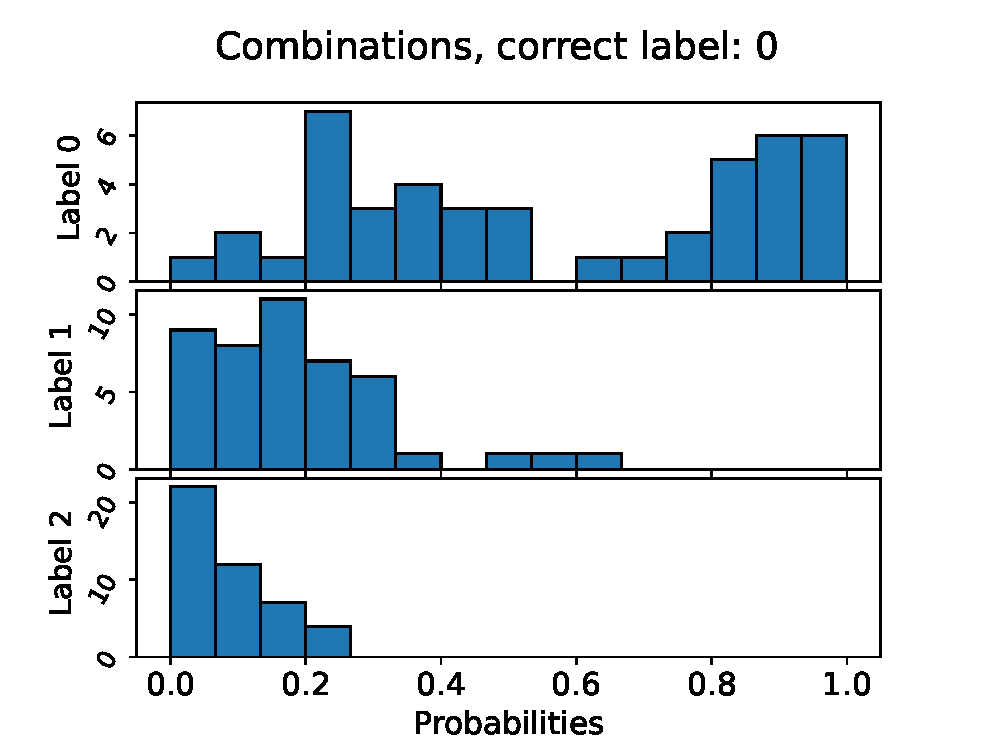
\includegraphics[width=\textwidth]{files/figs/app/hists/pelvis/c0.eps}
\end{minipage}%
\begin{minipage}{0.33\textwidth}
  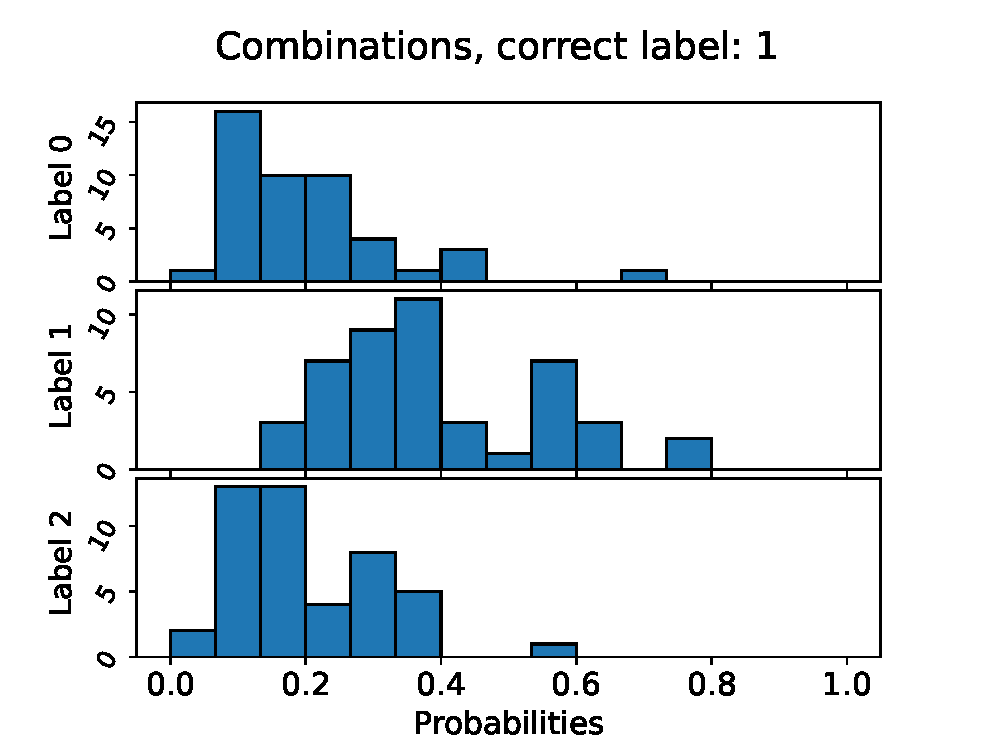
\includegraphics[width=\textwidth]{files/figs/app/hists/pelvis/c1.eps}
\end{minipage}%
\begin{minipage}{0.33\textwidth}
  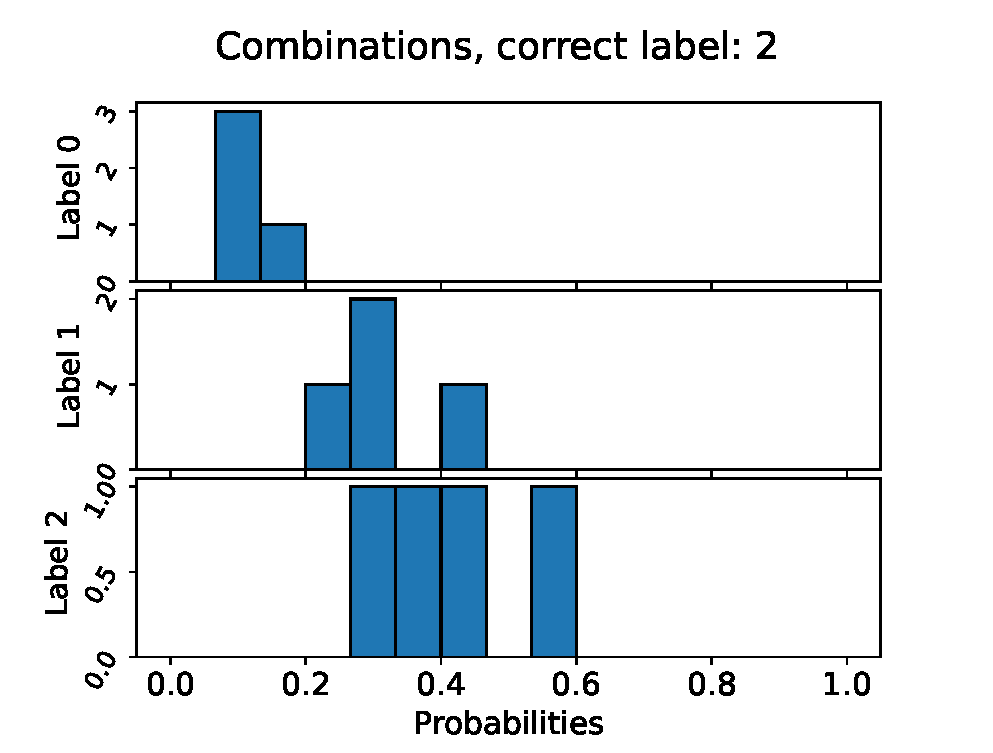
\includegraphics[width=\textwidth]{files/figs/app/hists/pelvis/c2.eps}
\end{minipage}

\begin{minipage}{0.33\textwidth}
  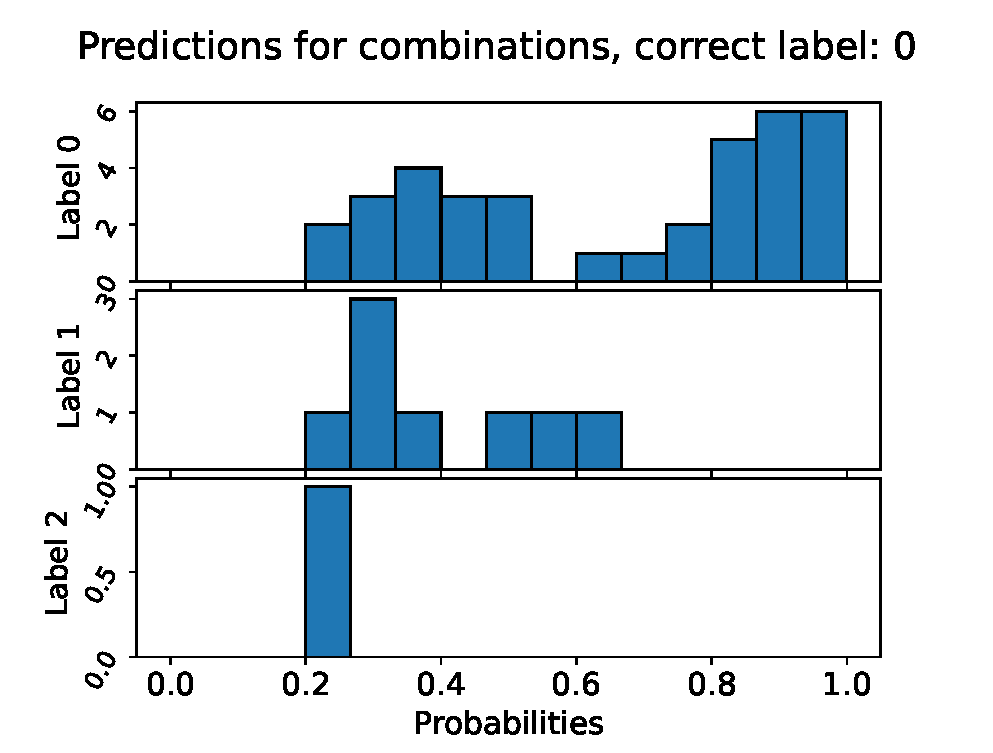
\includegraphics[width=\textwidth]{files/figs/app/hists/pelvis/pc0.eps}
\end{minipage}%
\begin{minipage}{0.33\textwidth}
  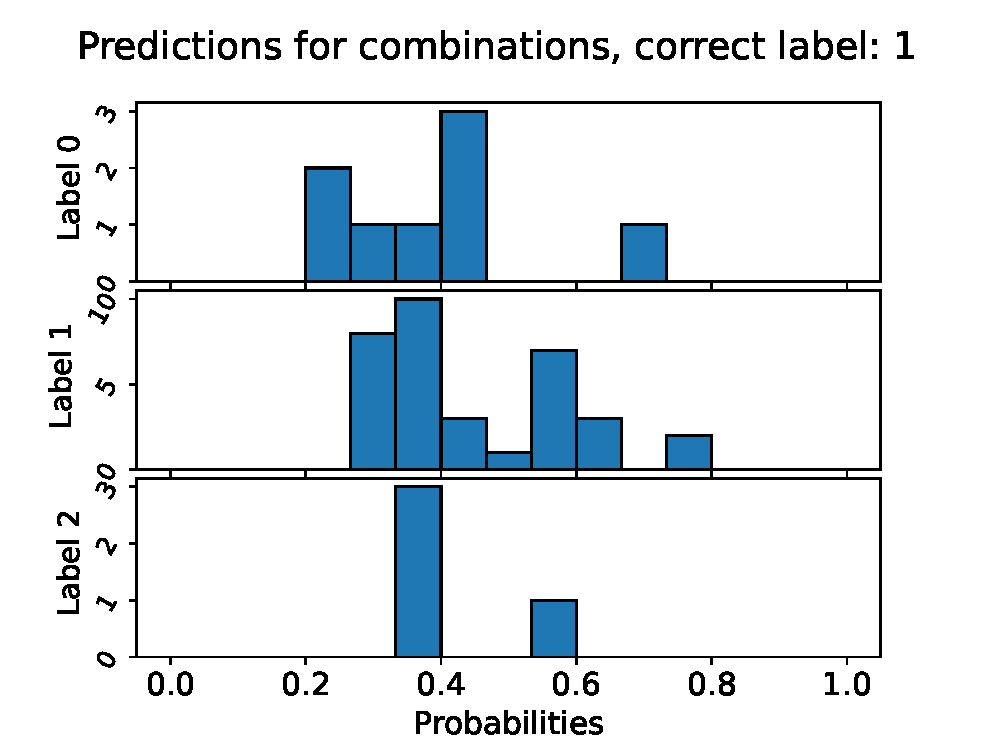
\includegraphics[width=\textwidth]{files/figs/app/hists/pelvis/pc1.eps}
\end{minipage}%
\begin{minipage}{0.33\textwidth}
  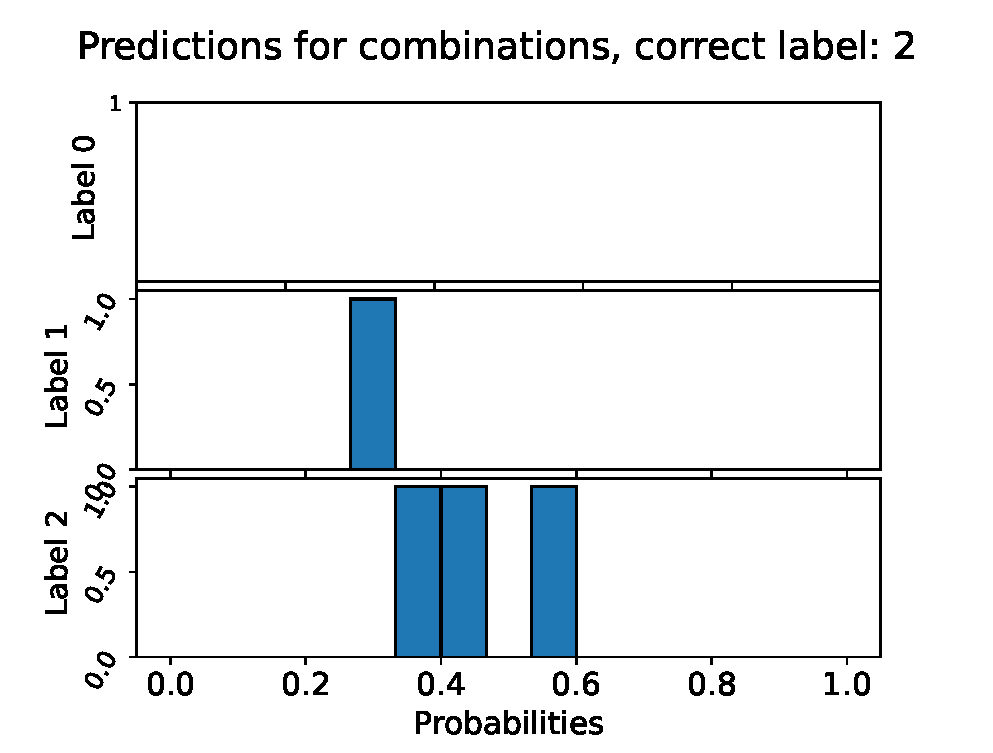
\includegraphics[width=\textwidth]{files/figs/app/hists/pelvis/pc2.eps}
\end{minipage}
\end{center}

\newpage
\section{Femoral Valgus}
The first row shows all the predicted probabilities for the different classes. The second row shows the probabilities for the predicted class for all repetitions, i.e. the histograms of the highest probabilities for the different classes for all repetitions. The third and fourth rows show the corresponding histograms for the combined scores.

\begin{center}
\begin{minipage}{0.33\textwidth}
  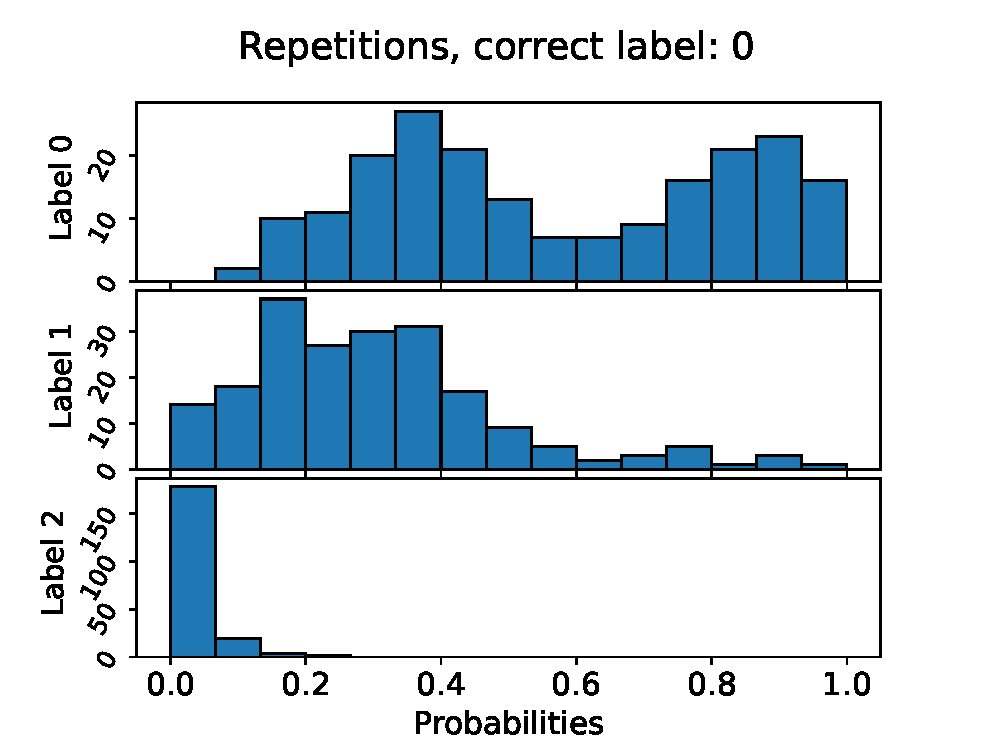
\includegraphics[width=\textwidth]{files/figs/app/hists/femval/r0.eps}
\end{minipage}%
\begin{minipage}{0.33\textwidth}
  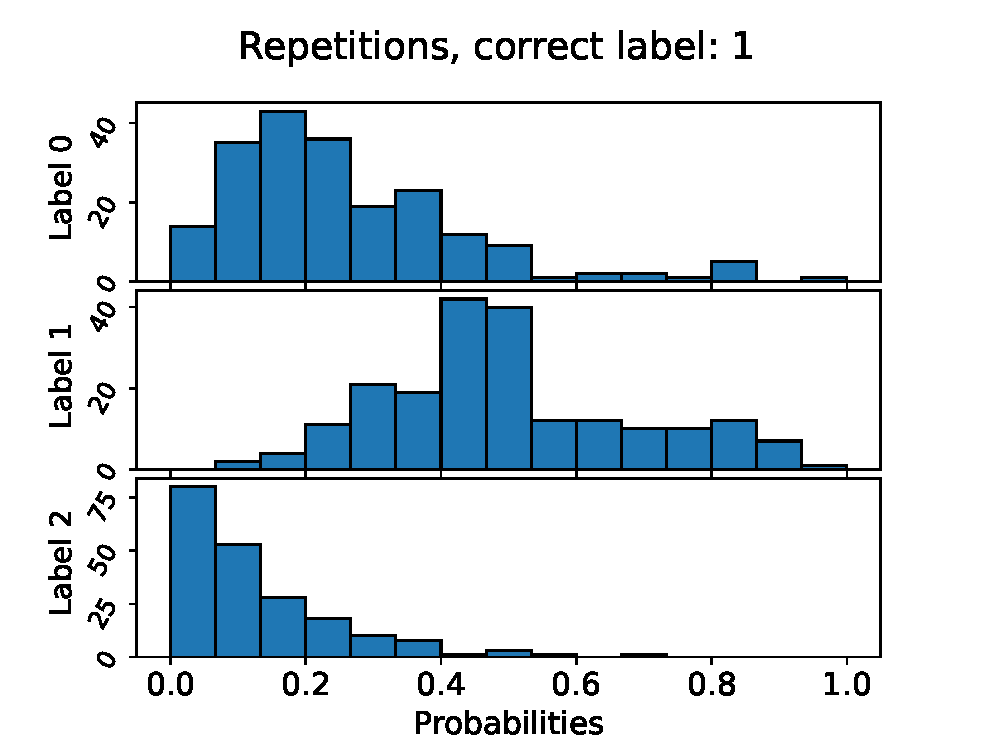
\includegraphics[width=\textwidth]{files/figs/app/hists/femval/r1.eps}
\end{minipage}%
\begin{minipage}{0.33\textwidth}
  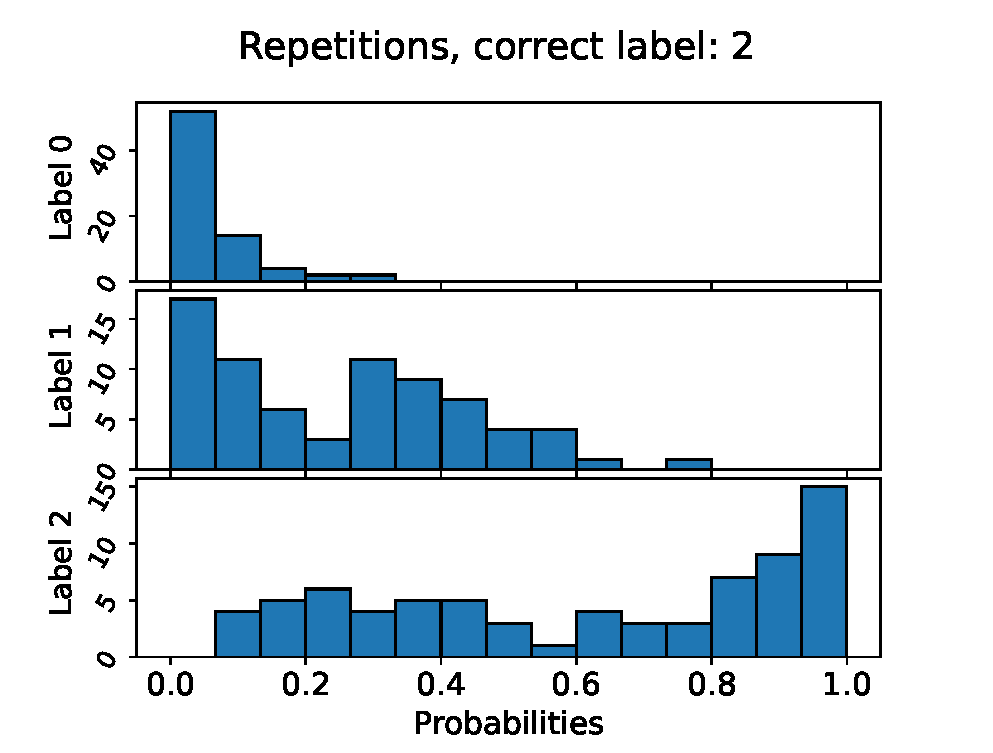
\includegraphics[width=\textwidth]{files/figs/app/hists/femval/r2.eps}
\end{minipage}

\begin{minipage}{0.33\textwidth}
  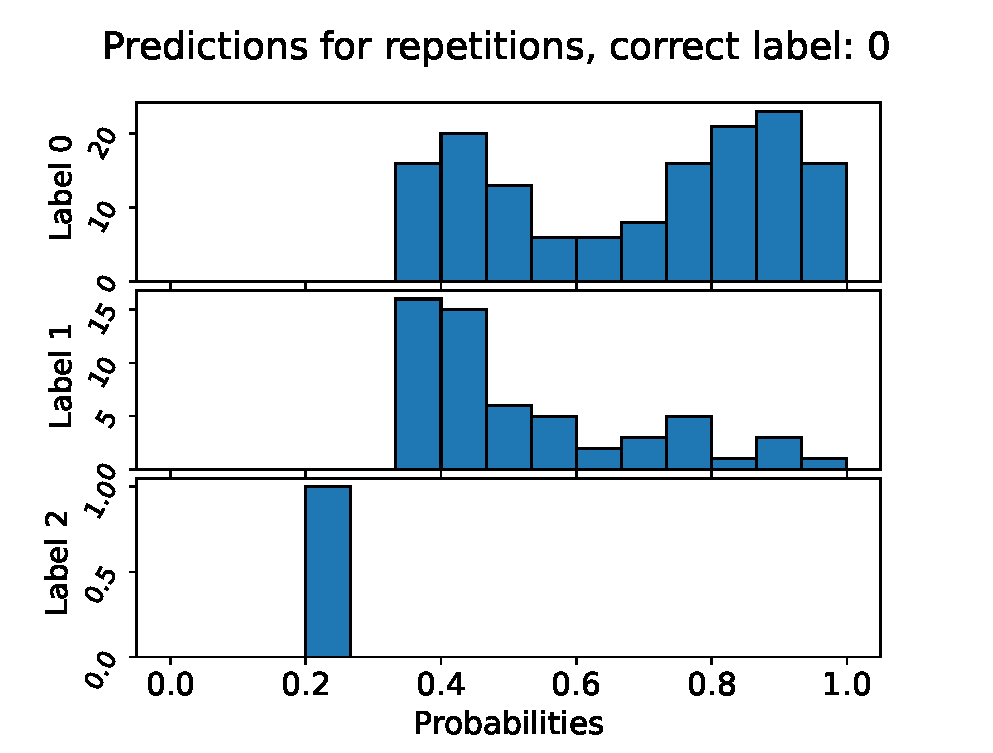
\includegraphics[width=\textwidth]{files/figs/app/hists/femval/pr0.eps}
\end{minipage}%
\begin{minipage}{0.33\textwidth}
  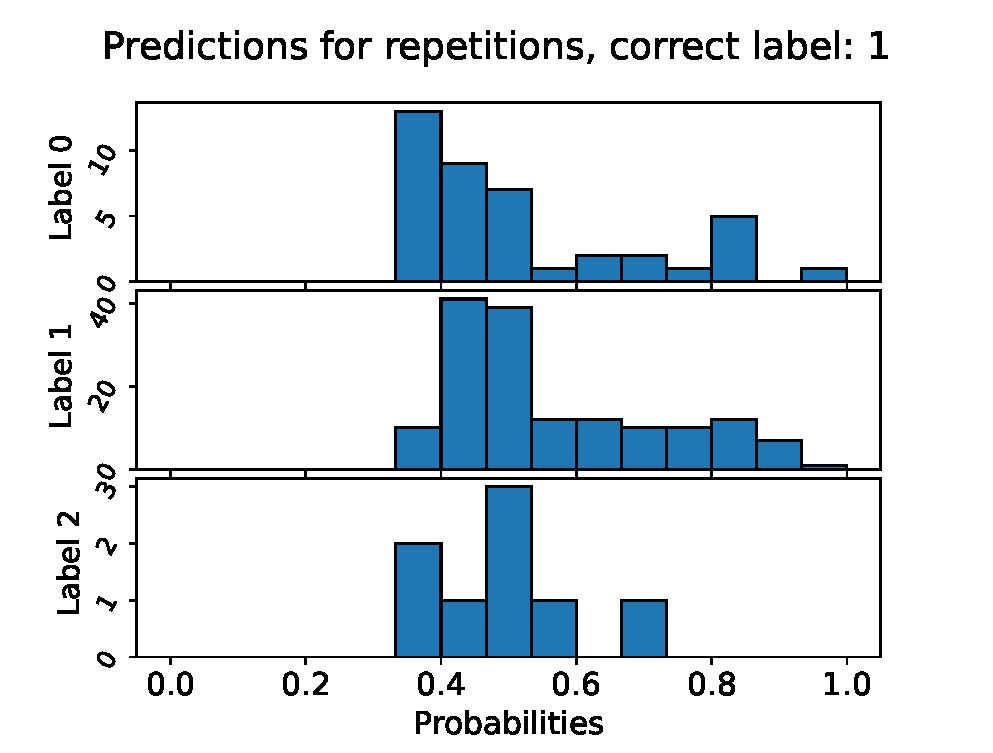
\includegraphics[width=\textwidth]{files/figs/app/hists/femval/pr1.eps}
\end{minipage}%
\begin{minipage}{0.33\textwidth}
  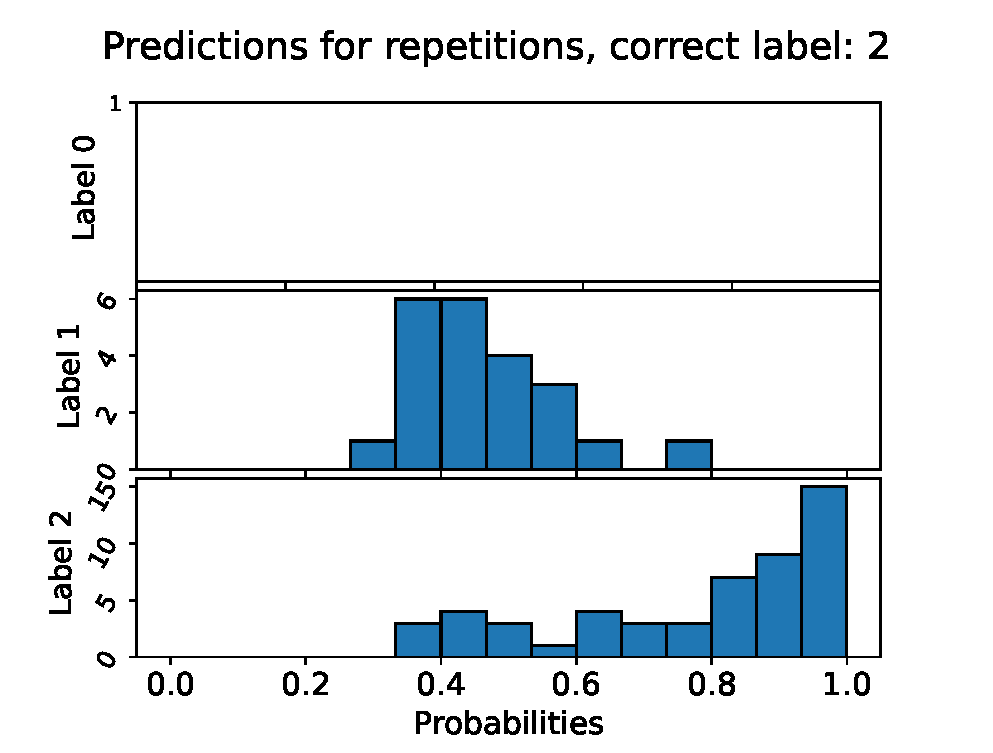
\includegraphics[width=\textwidth]{files/figs/app/hists/femval/pr2.eps}
\end{minipage}

\begin{minipage}{0.33\textwidth}
  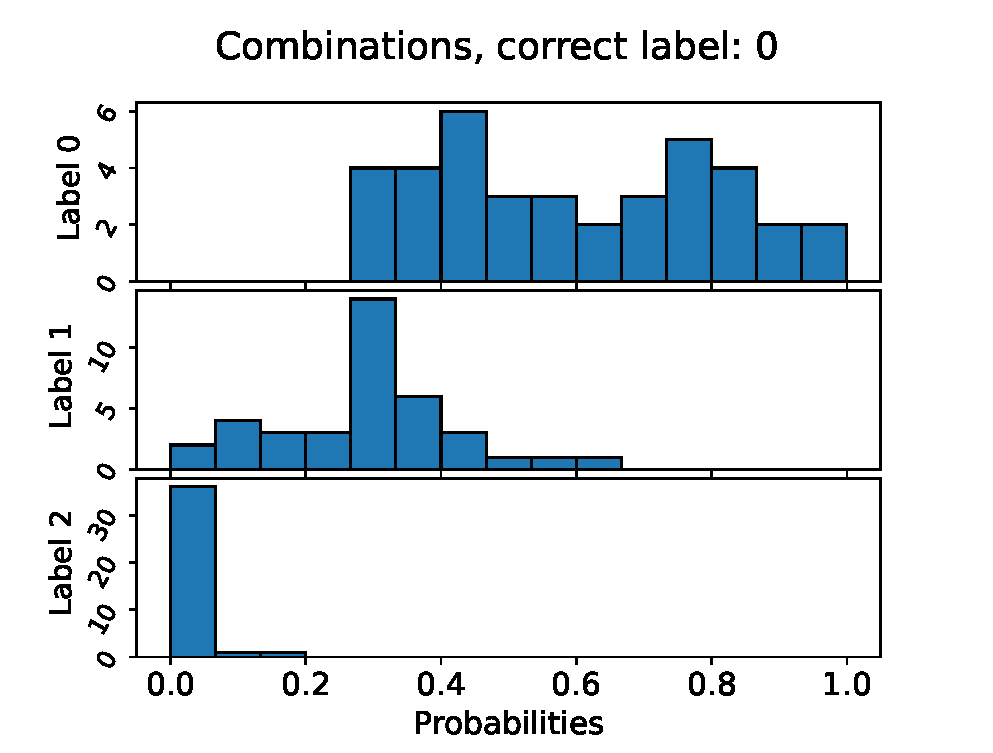
\includegraphics[width=\textwidth]{files/figs/app/hists/femval/c0.eps}
\end{minipage}%
\begin{minipage}{0.33\textwidth}
  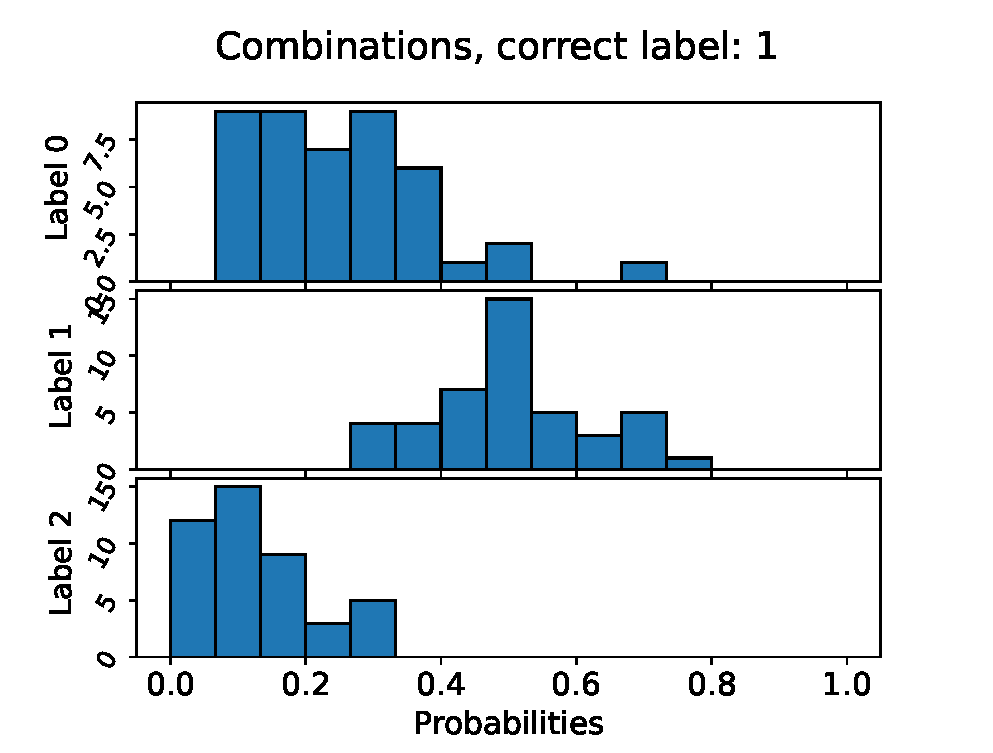
\includegraphics[width=\textwidth]{files/figs/app/hists/femval/c1.eps}
\end{minipage}%
\begin{minipage}{0.33\textwidth}
  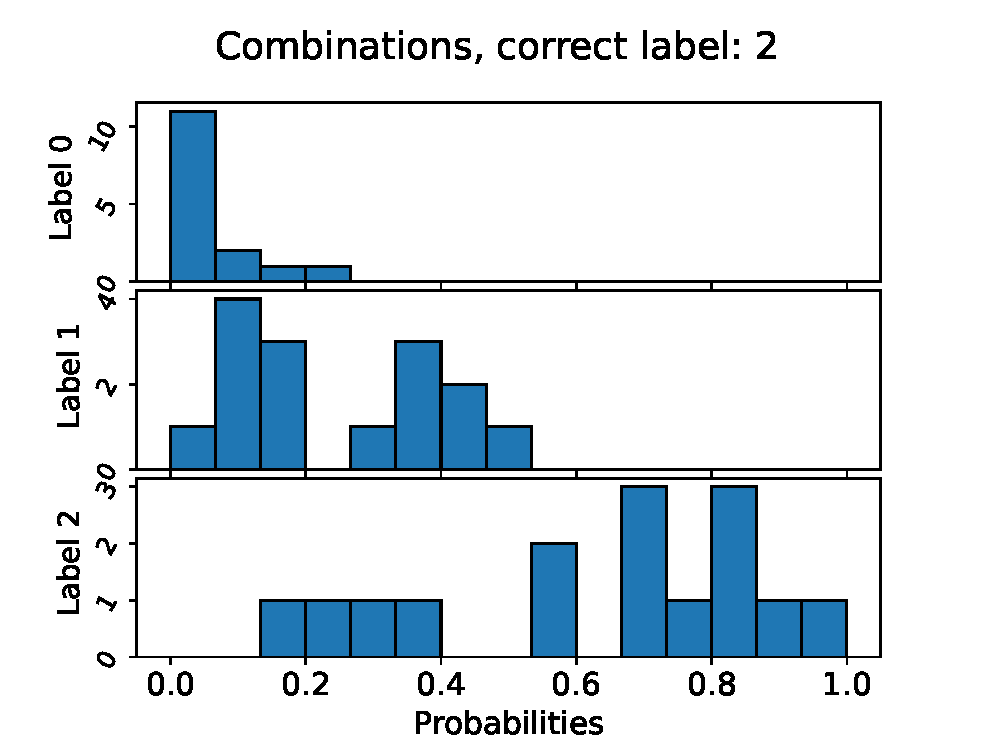
\includegraphics[width=\textwidth]{files/figs/app/hists/femval/c2.eps}
\end{minipage}

\begin{minipage}{0.33\textwidth}
  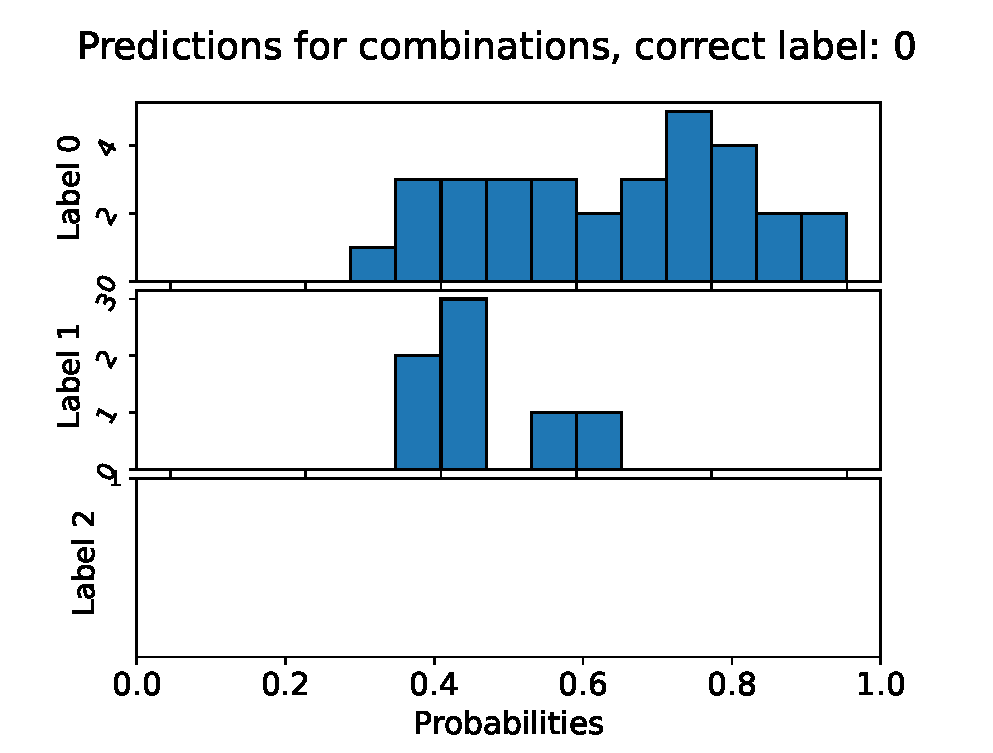
\includegraphics[width=\textwidth]{files/figs/app/hists/femval/pc0.eps}
\end{minipage}%
\begin{minipage}{0.33\textwidth}
  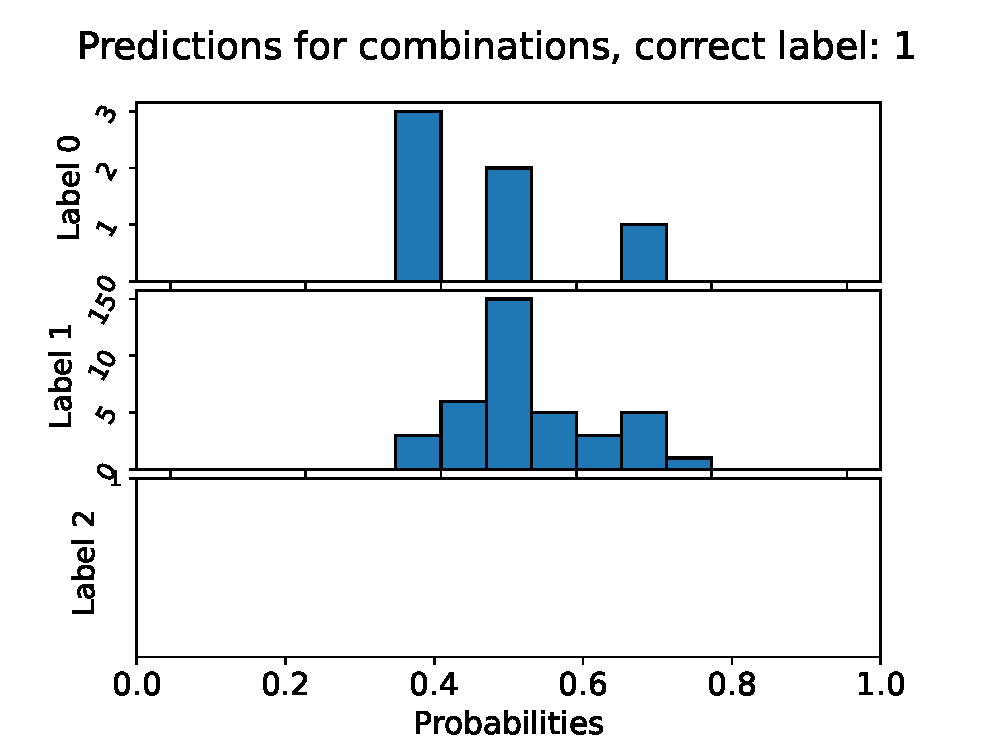
\includegraphics[width=\textwidth]{files/figs/app/hists/femval/pc1.eps}
\end{minipage}%
\begin{minipage}{0.33\textwidth}
  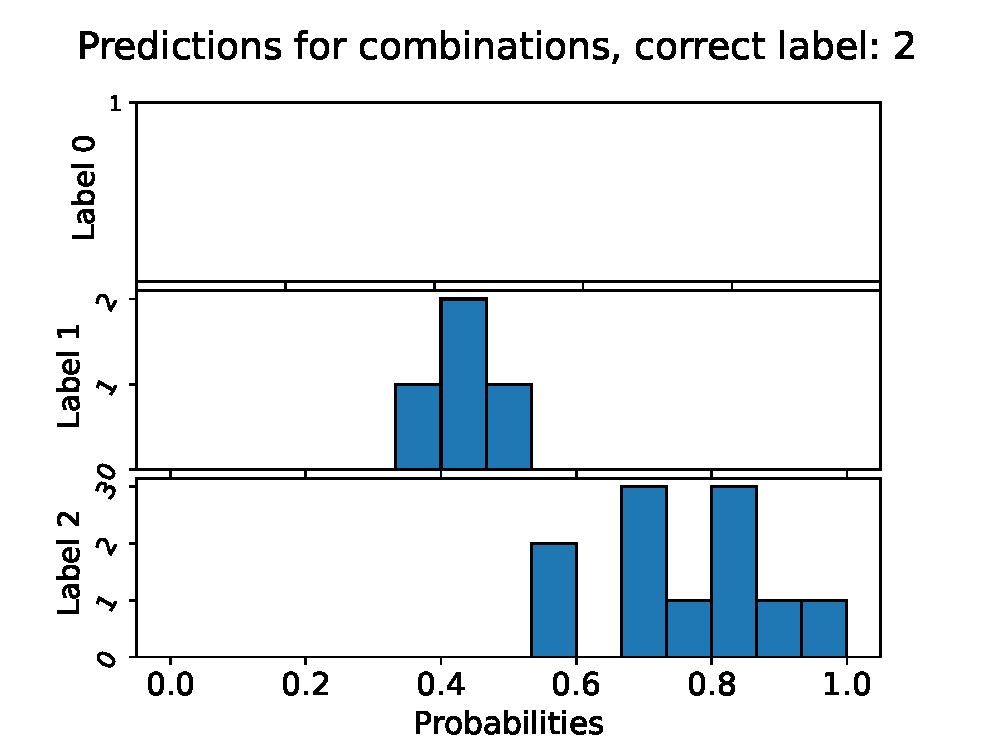
\includegraphics[width=\textwidth]{files/figs/app/hists/femval/pc2.eps}
\end{minipage}
\end{center}

\newpage
\section{Knee Medial-to-Foot Position}
The first row shows all the predicted probabilities for the different classes. The second row shows the probabilities for the predicted class for all repetitions, i.e. the histograms of the highest probabilities for the different classes for all repetitions. The third and fourth rows show the corresponding histograms for the combined scores.


\begin{center}
\begin{minipage}{0.33\textwidth}
  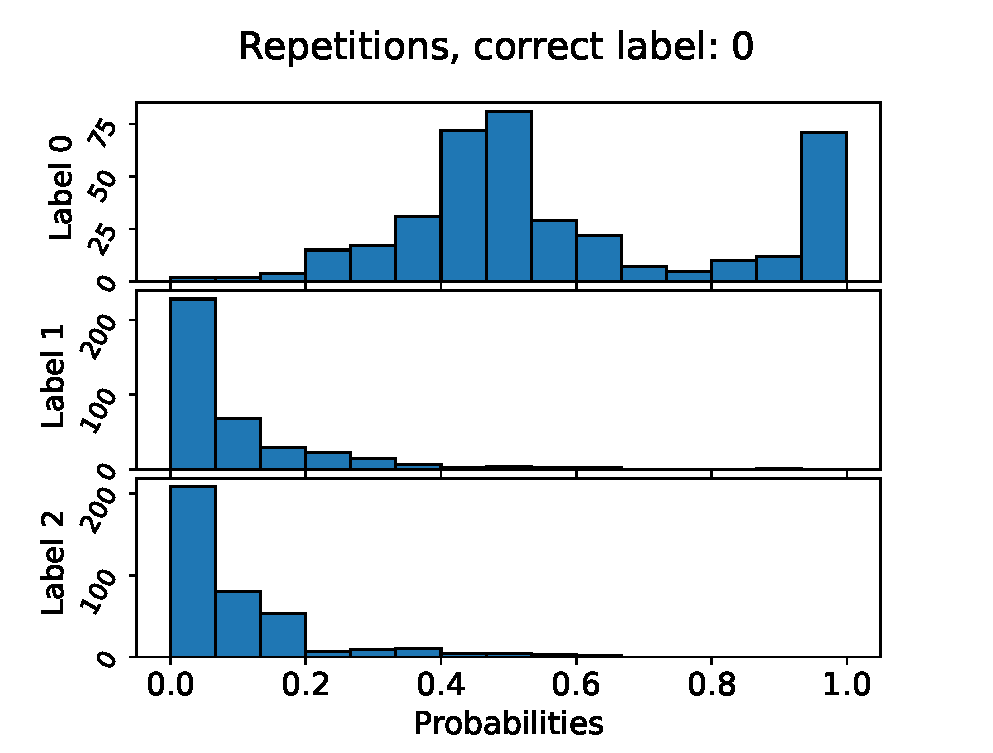
\includegraphics[width=\textwidth]{files/figs/app/hists/kmfp/r0.eps}
\end{minipage}%
\begin{minipage}{0.33\textwidth}
  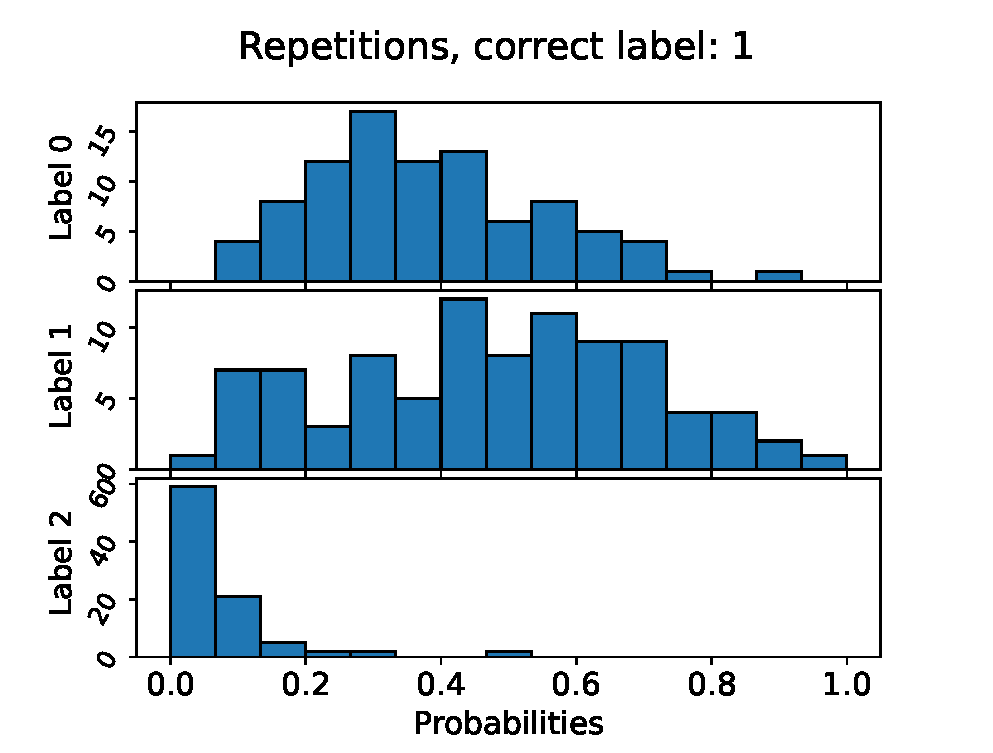
\includegraphics[width=\textwidth]{files/figs/app/hists/kmfp/r1.eps}
\end{minipage}%
\begin{minipage}{0.33\textwidth}
  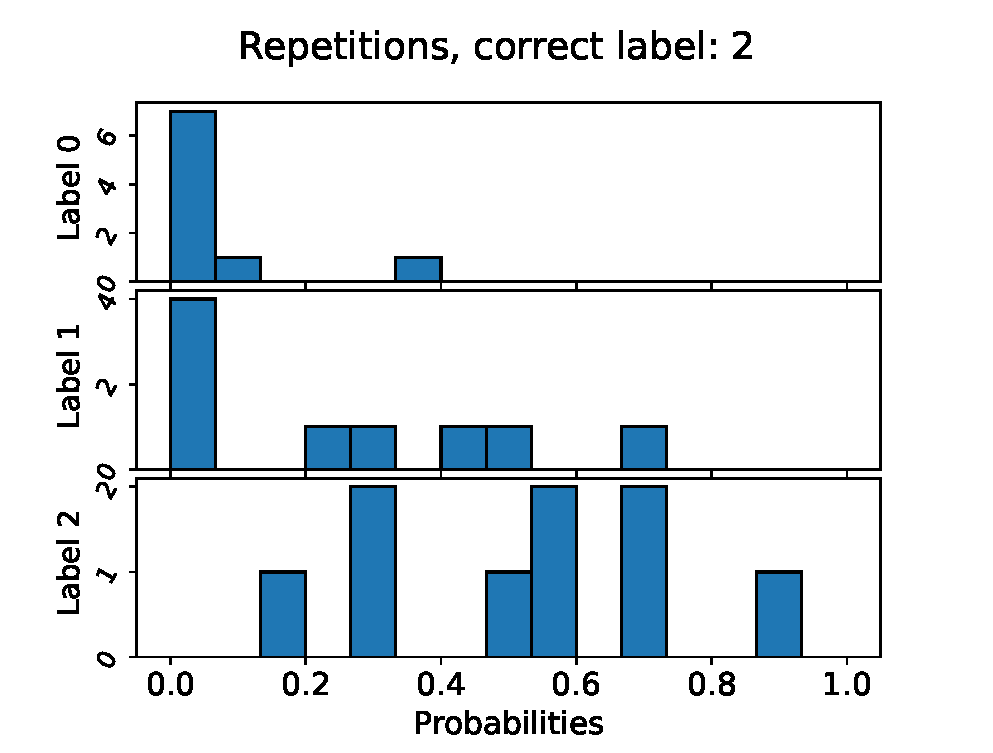
\includegraphics[width=\textwidth]{files/figs/app/hists/kmfp/r2.eps}
\end{minipage}

\begin{minipage}{0.33\textwidth}
  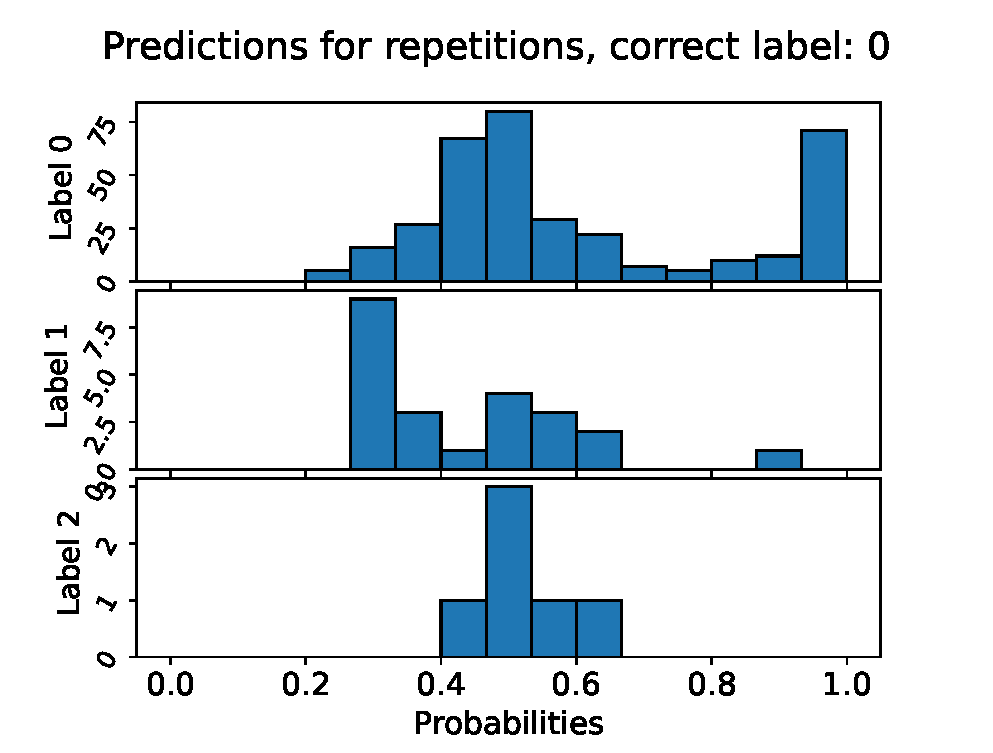
\includegraphics[width=\textwidth]{files/figs/app/hists/kmfp/pr0.eps}
\end{minipage}%
\begin{minipage}{0.33\textwidth}
  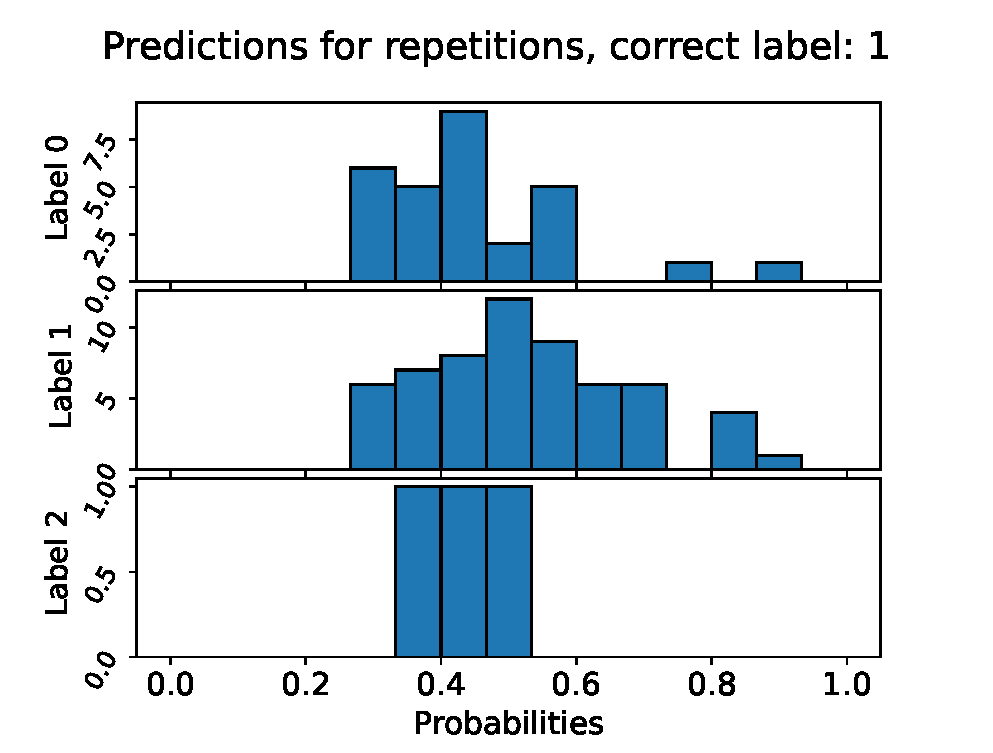
\includegraphics[width=\textwidth]{files/figs/app/hists/kmfp/pr1.eps}
\end{minipage}%
\begin{minipage}{0.33\textwidth}
  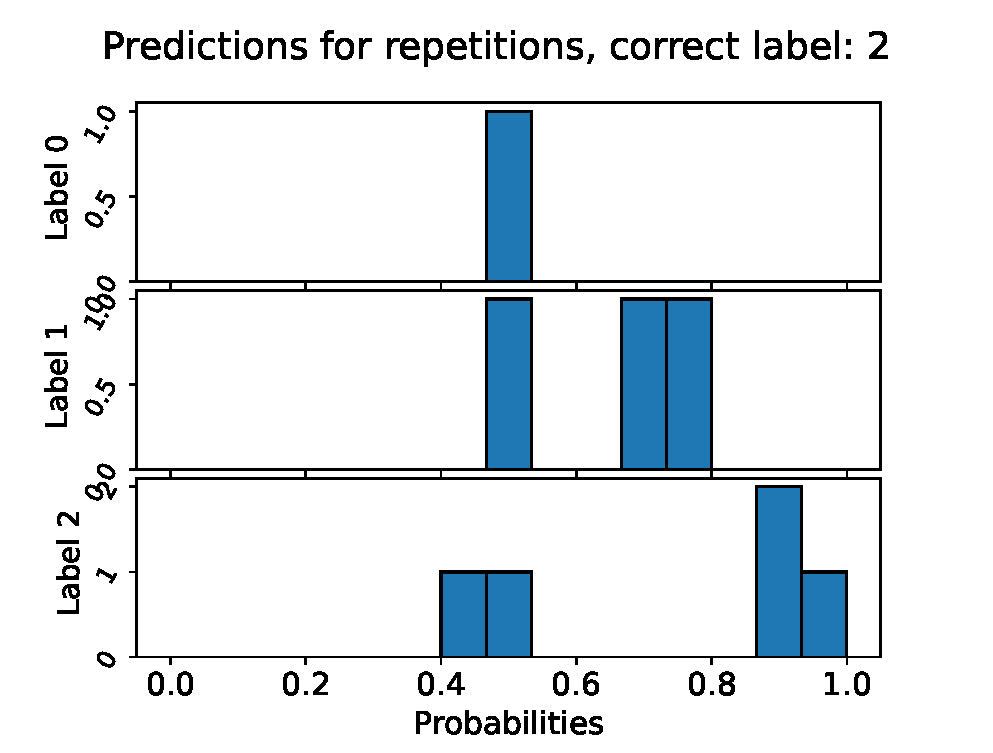
\includegraphics[width=\textwidth]{files/figs/app/hists/kmfp/pr2.eps}
\end{minipage}

\begin{minipage}{0.33\textwidth}
  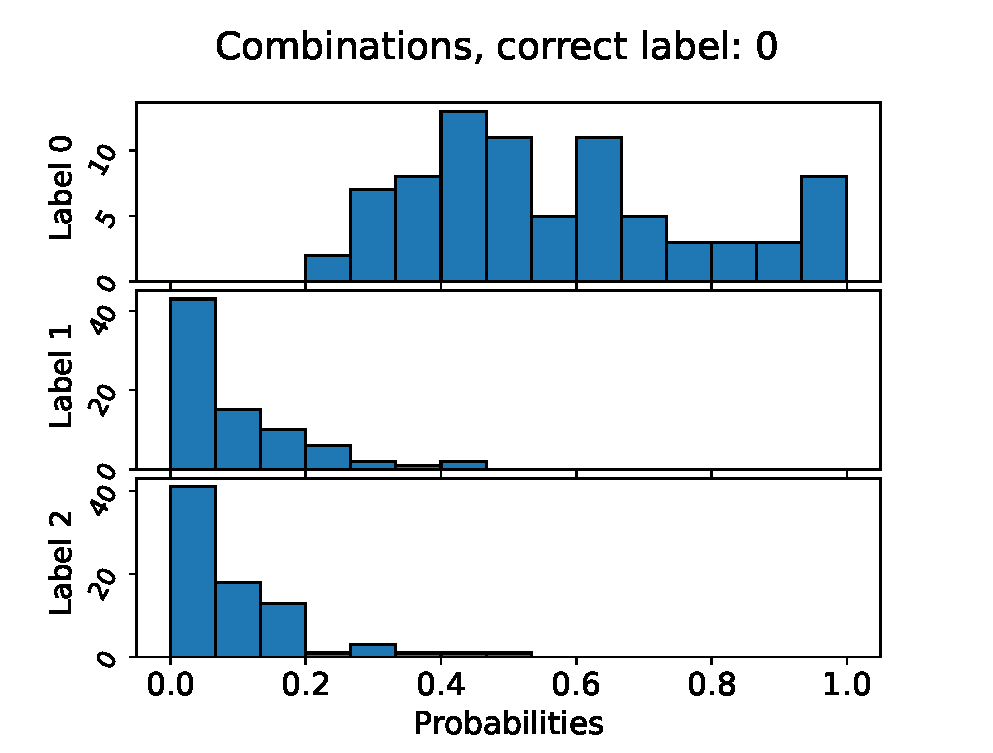
\includegraphics[width=\textwidth]{files/figs/app/hists/kmfp/c0.eps}
\end{minipage}%
\begin{minipage}{0.33\textwidth}
  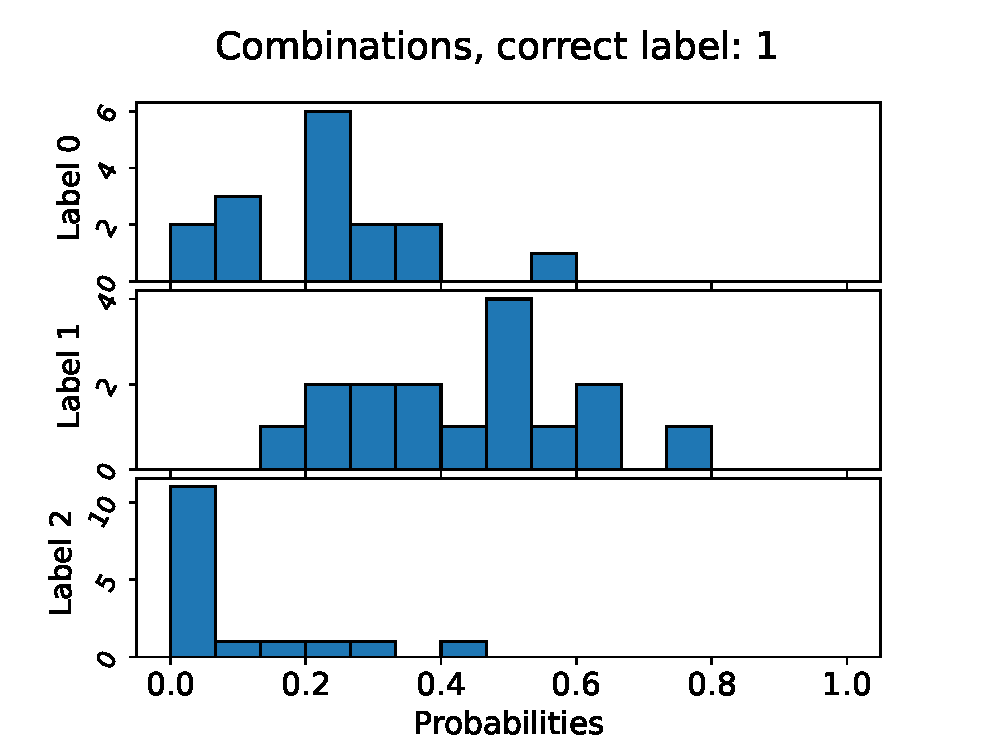
\includegraphics[width=\textwidth]{files/figs/app/hists/kmfp/c1.eps}
\end{minipage}%
\begin{minipage}{0.33\textwidth}
  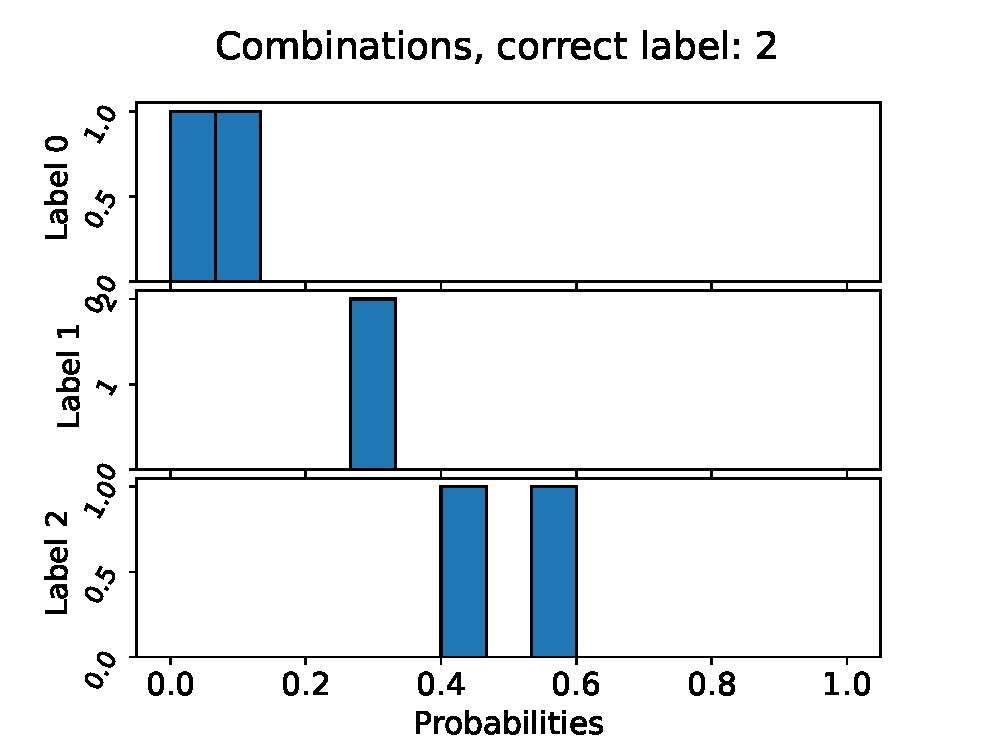
\includegraphics[width=\textwidth]{files/figs/app/hists/kmfp/c2.eps}
\end{minipage}

\begin{minipage}{0.33\textwidth}
  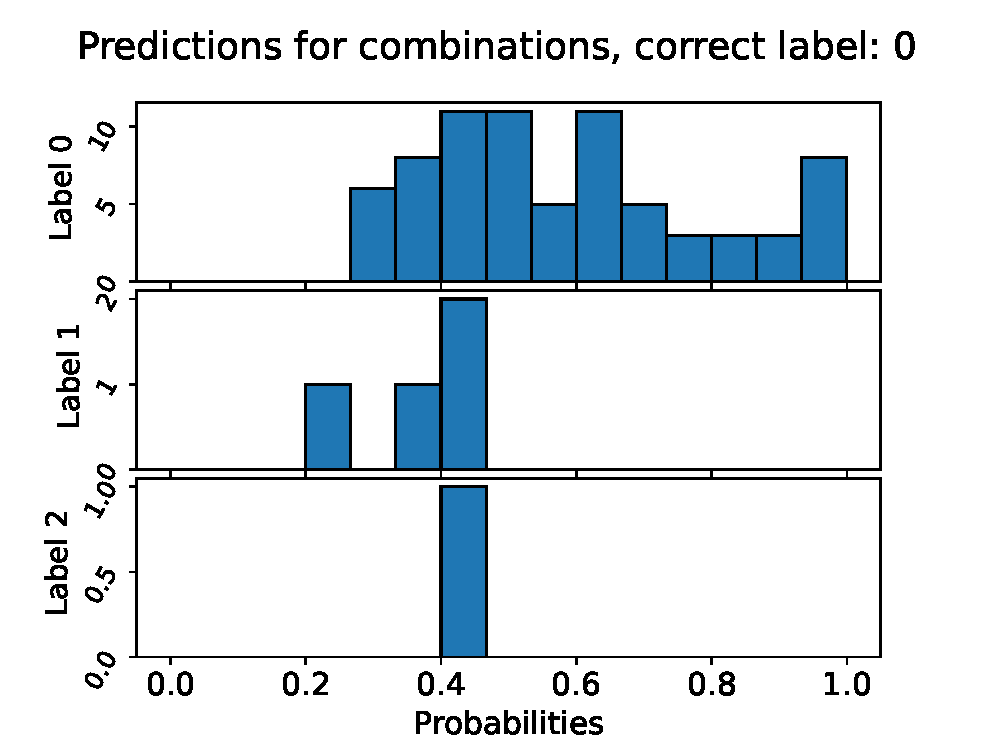
\includegraphics[width=\textwidth]{files/figs/app/hists/kmfp/pc0.eps}
\end{minipage}%
\begin{minipage}{0.33\textwidth}
  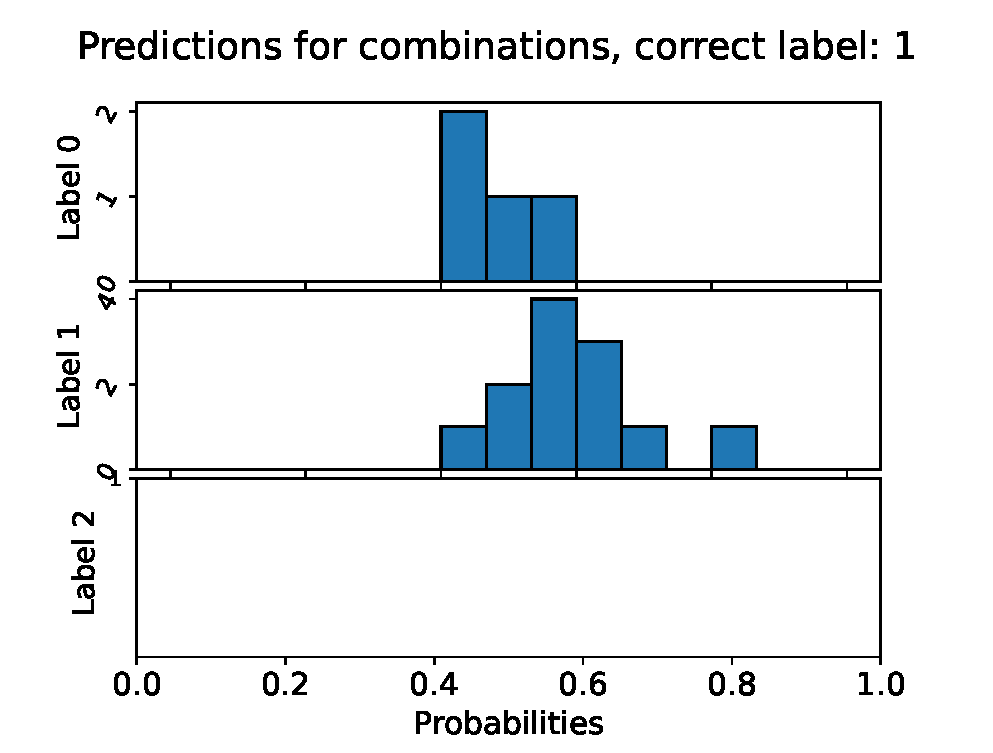
\includegraphics[width=\textwidth]{files/figs/app/hists/kmfp/pc1.eps}
\end{minipage}%
\begin{minipage}{0.33\textwidth}
  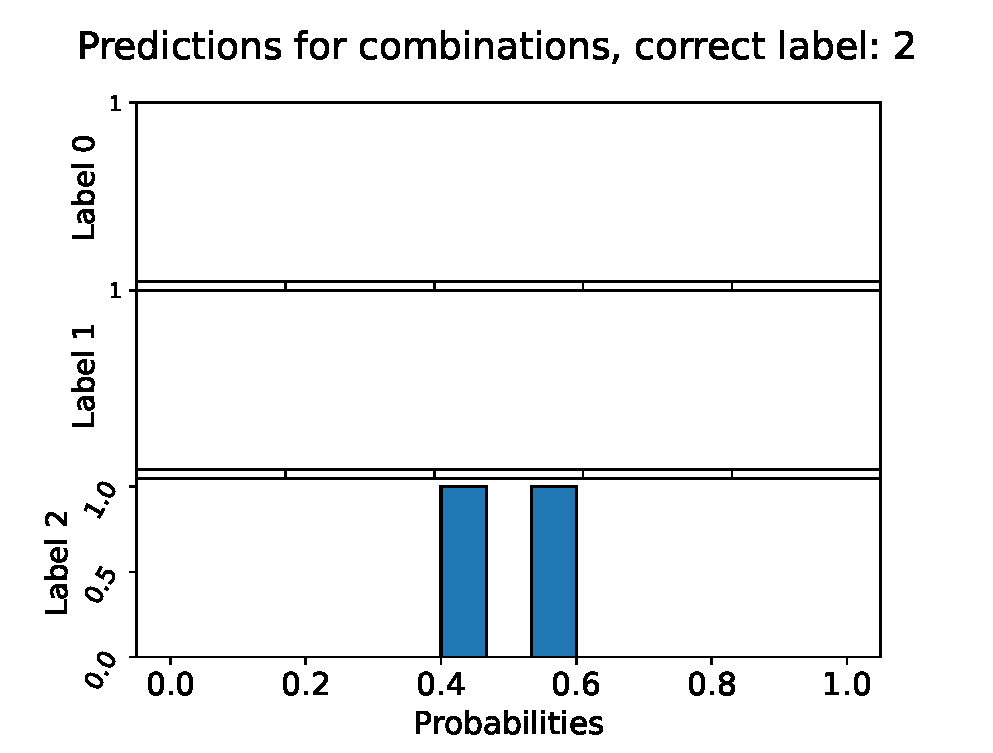
\includegraphics[width=\textwidth]{files/figs/app/hists/kmfp/pc2.eps}
\end{minipage}
\end{center}
